













%----------------------------------------------------------------------------------------

\newpage

%%%%%%%%%%%%%%%%%%%%%%%
\section{Aggregation-diffusion morphogenesis}{Morphogenèse par agrégation-diffusion}

\label{app:sec:density}




%%%%%%%%%%%%%%%%%%%%%%%
\subsection{Extended Figures for Model Exploration}{Figures supplémentaires pour l'exploration du modèle}


\subsubsection{Convergence}{Convergence}

Histograms for the 81 parameters points for which we did 100 repetitions are given in Fig.~\ref{fig:histograms}, for Moran index and slope indicators. Other indicators showed similar convergence patterns. The visual exploration of histograms confirms the numerical analysis done in main text for statistical convergence.

% histograms


% and bimodal statistical distribution for cumulated points in the parameter space confirm the existence of superposed regimes : gaussian distribution gives stationary configurations, whereas inverse log-normal distribution are close to real data shape and correspond to non-stationary regime.
% -> not sure it is interesting to look at cumulated histograms.

% Figures :

%%%%%%%%%%%%%%%%%%%%
\begin{figure}
\centering
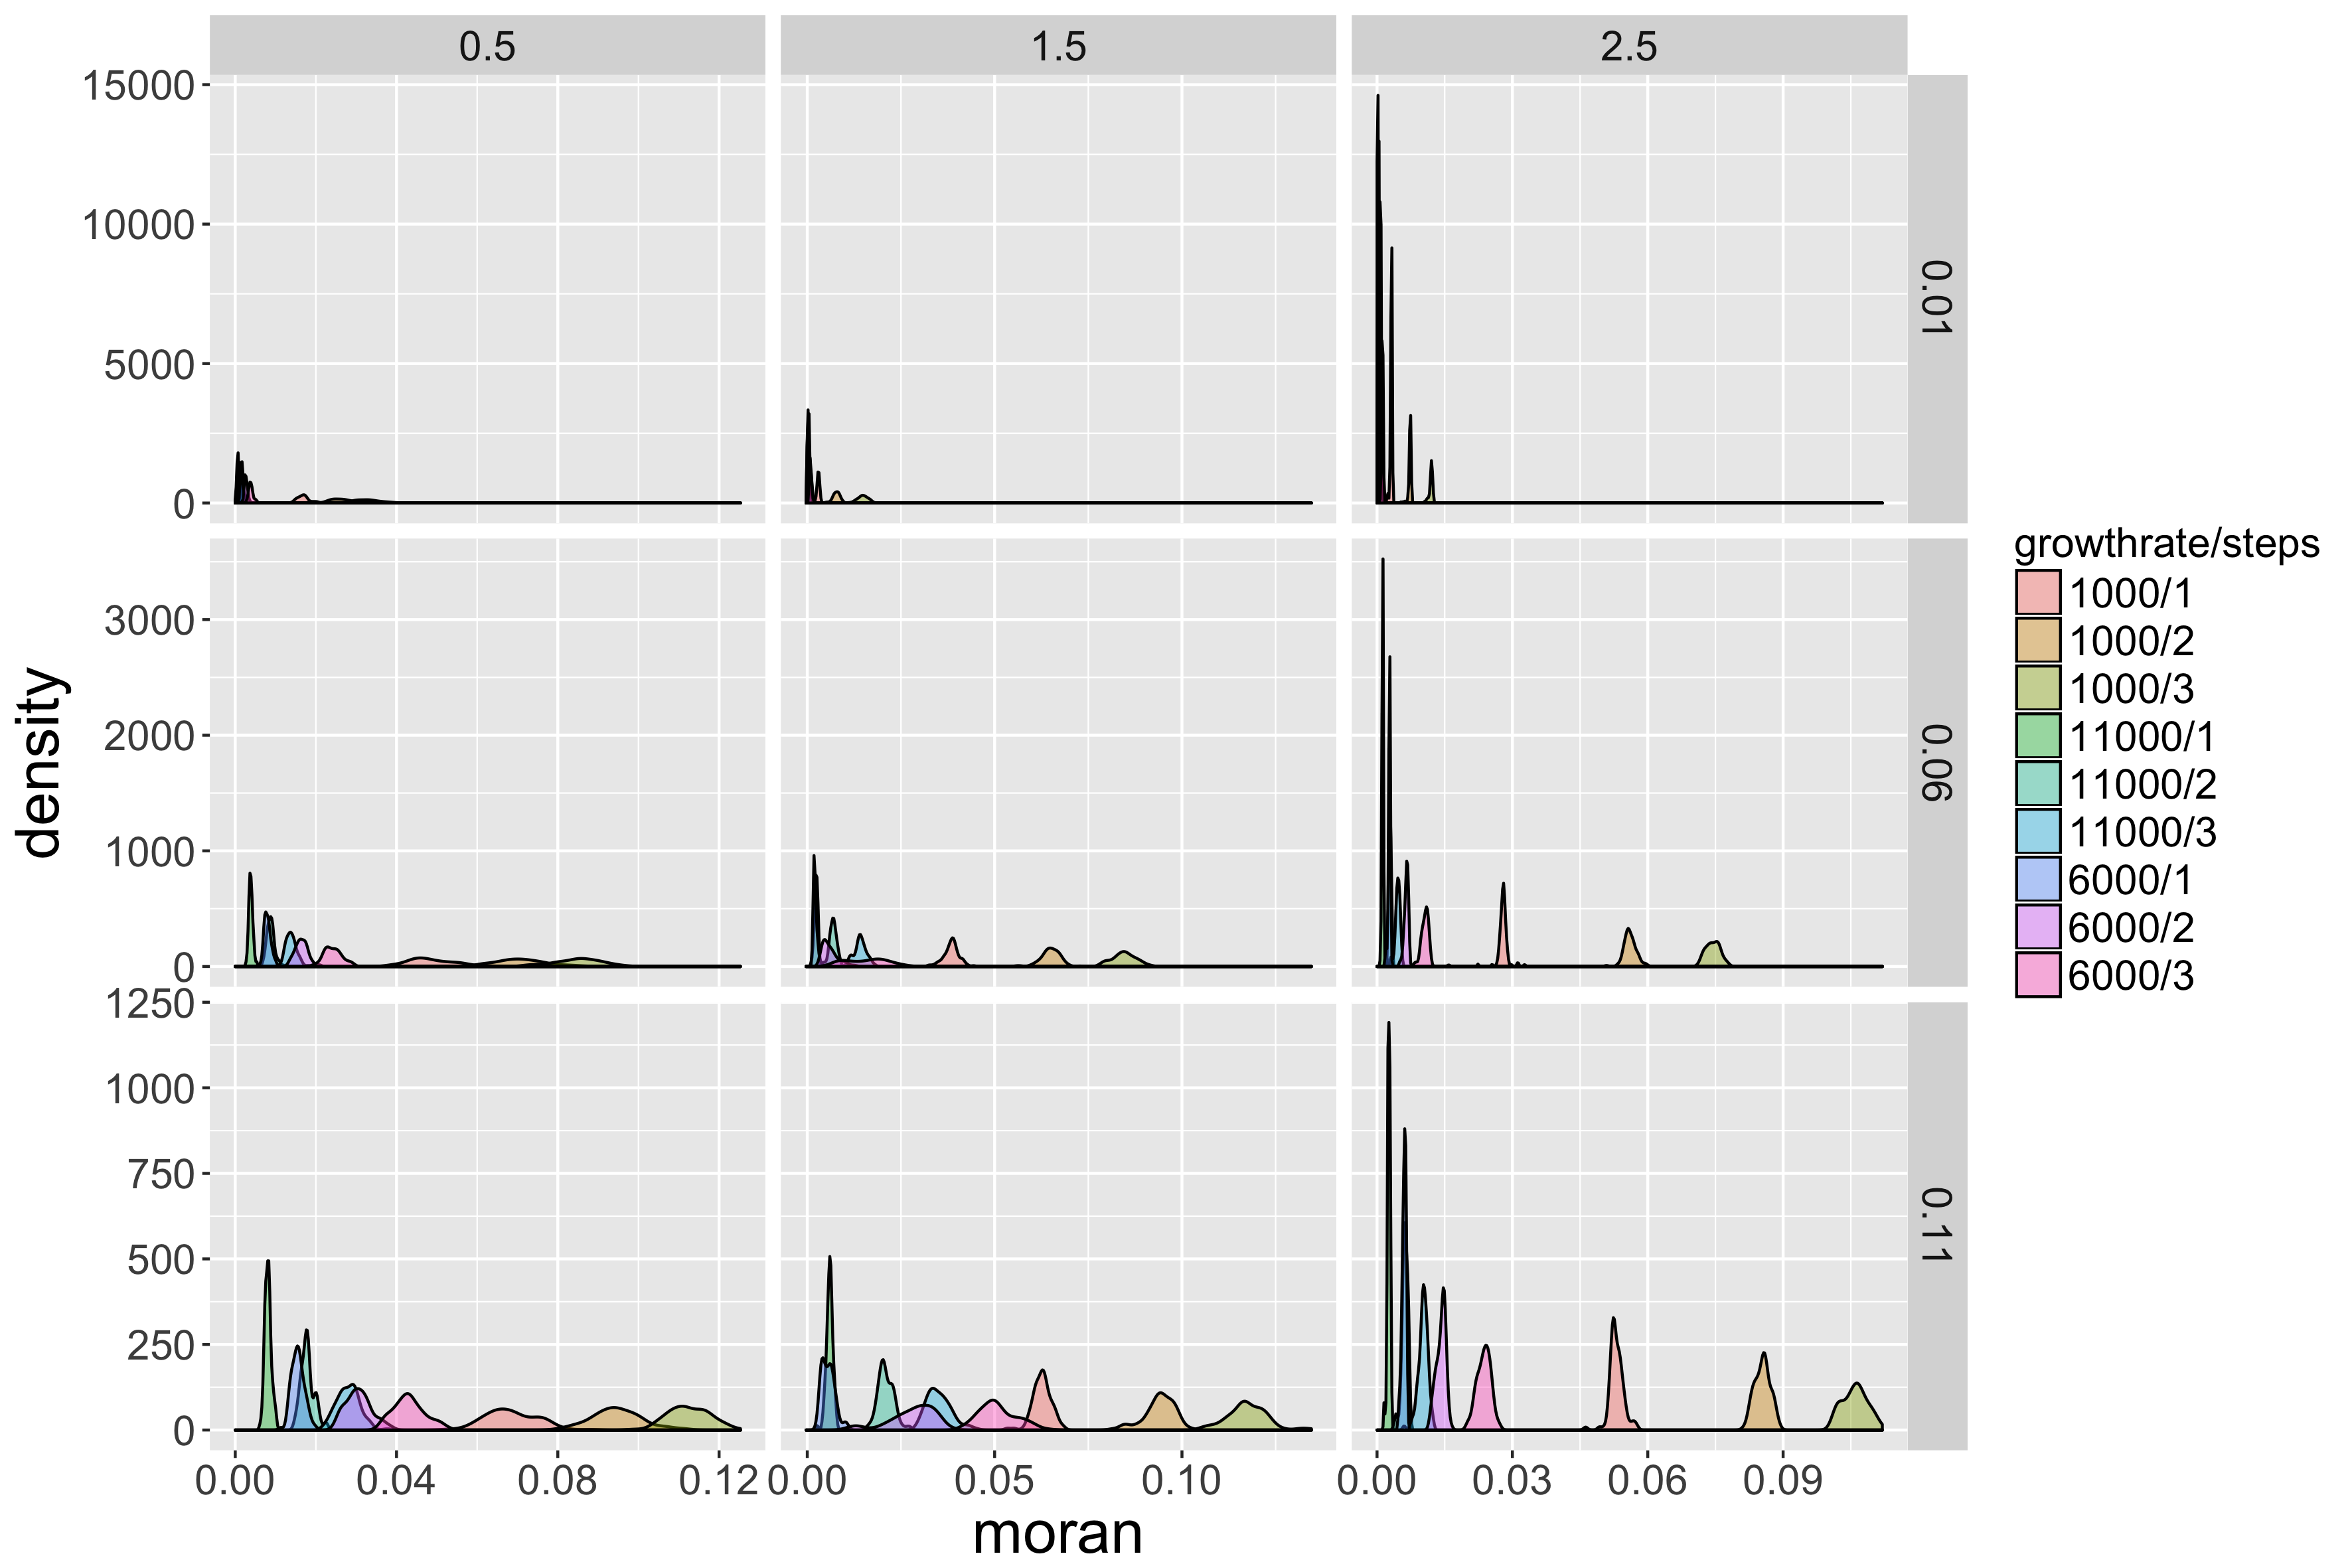
\includegraphics[width=0.8\textwidth]{Figures/Density/hist_moran}\\
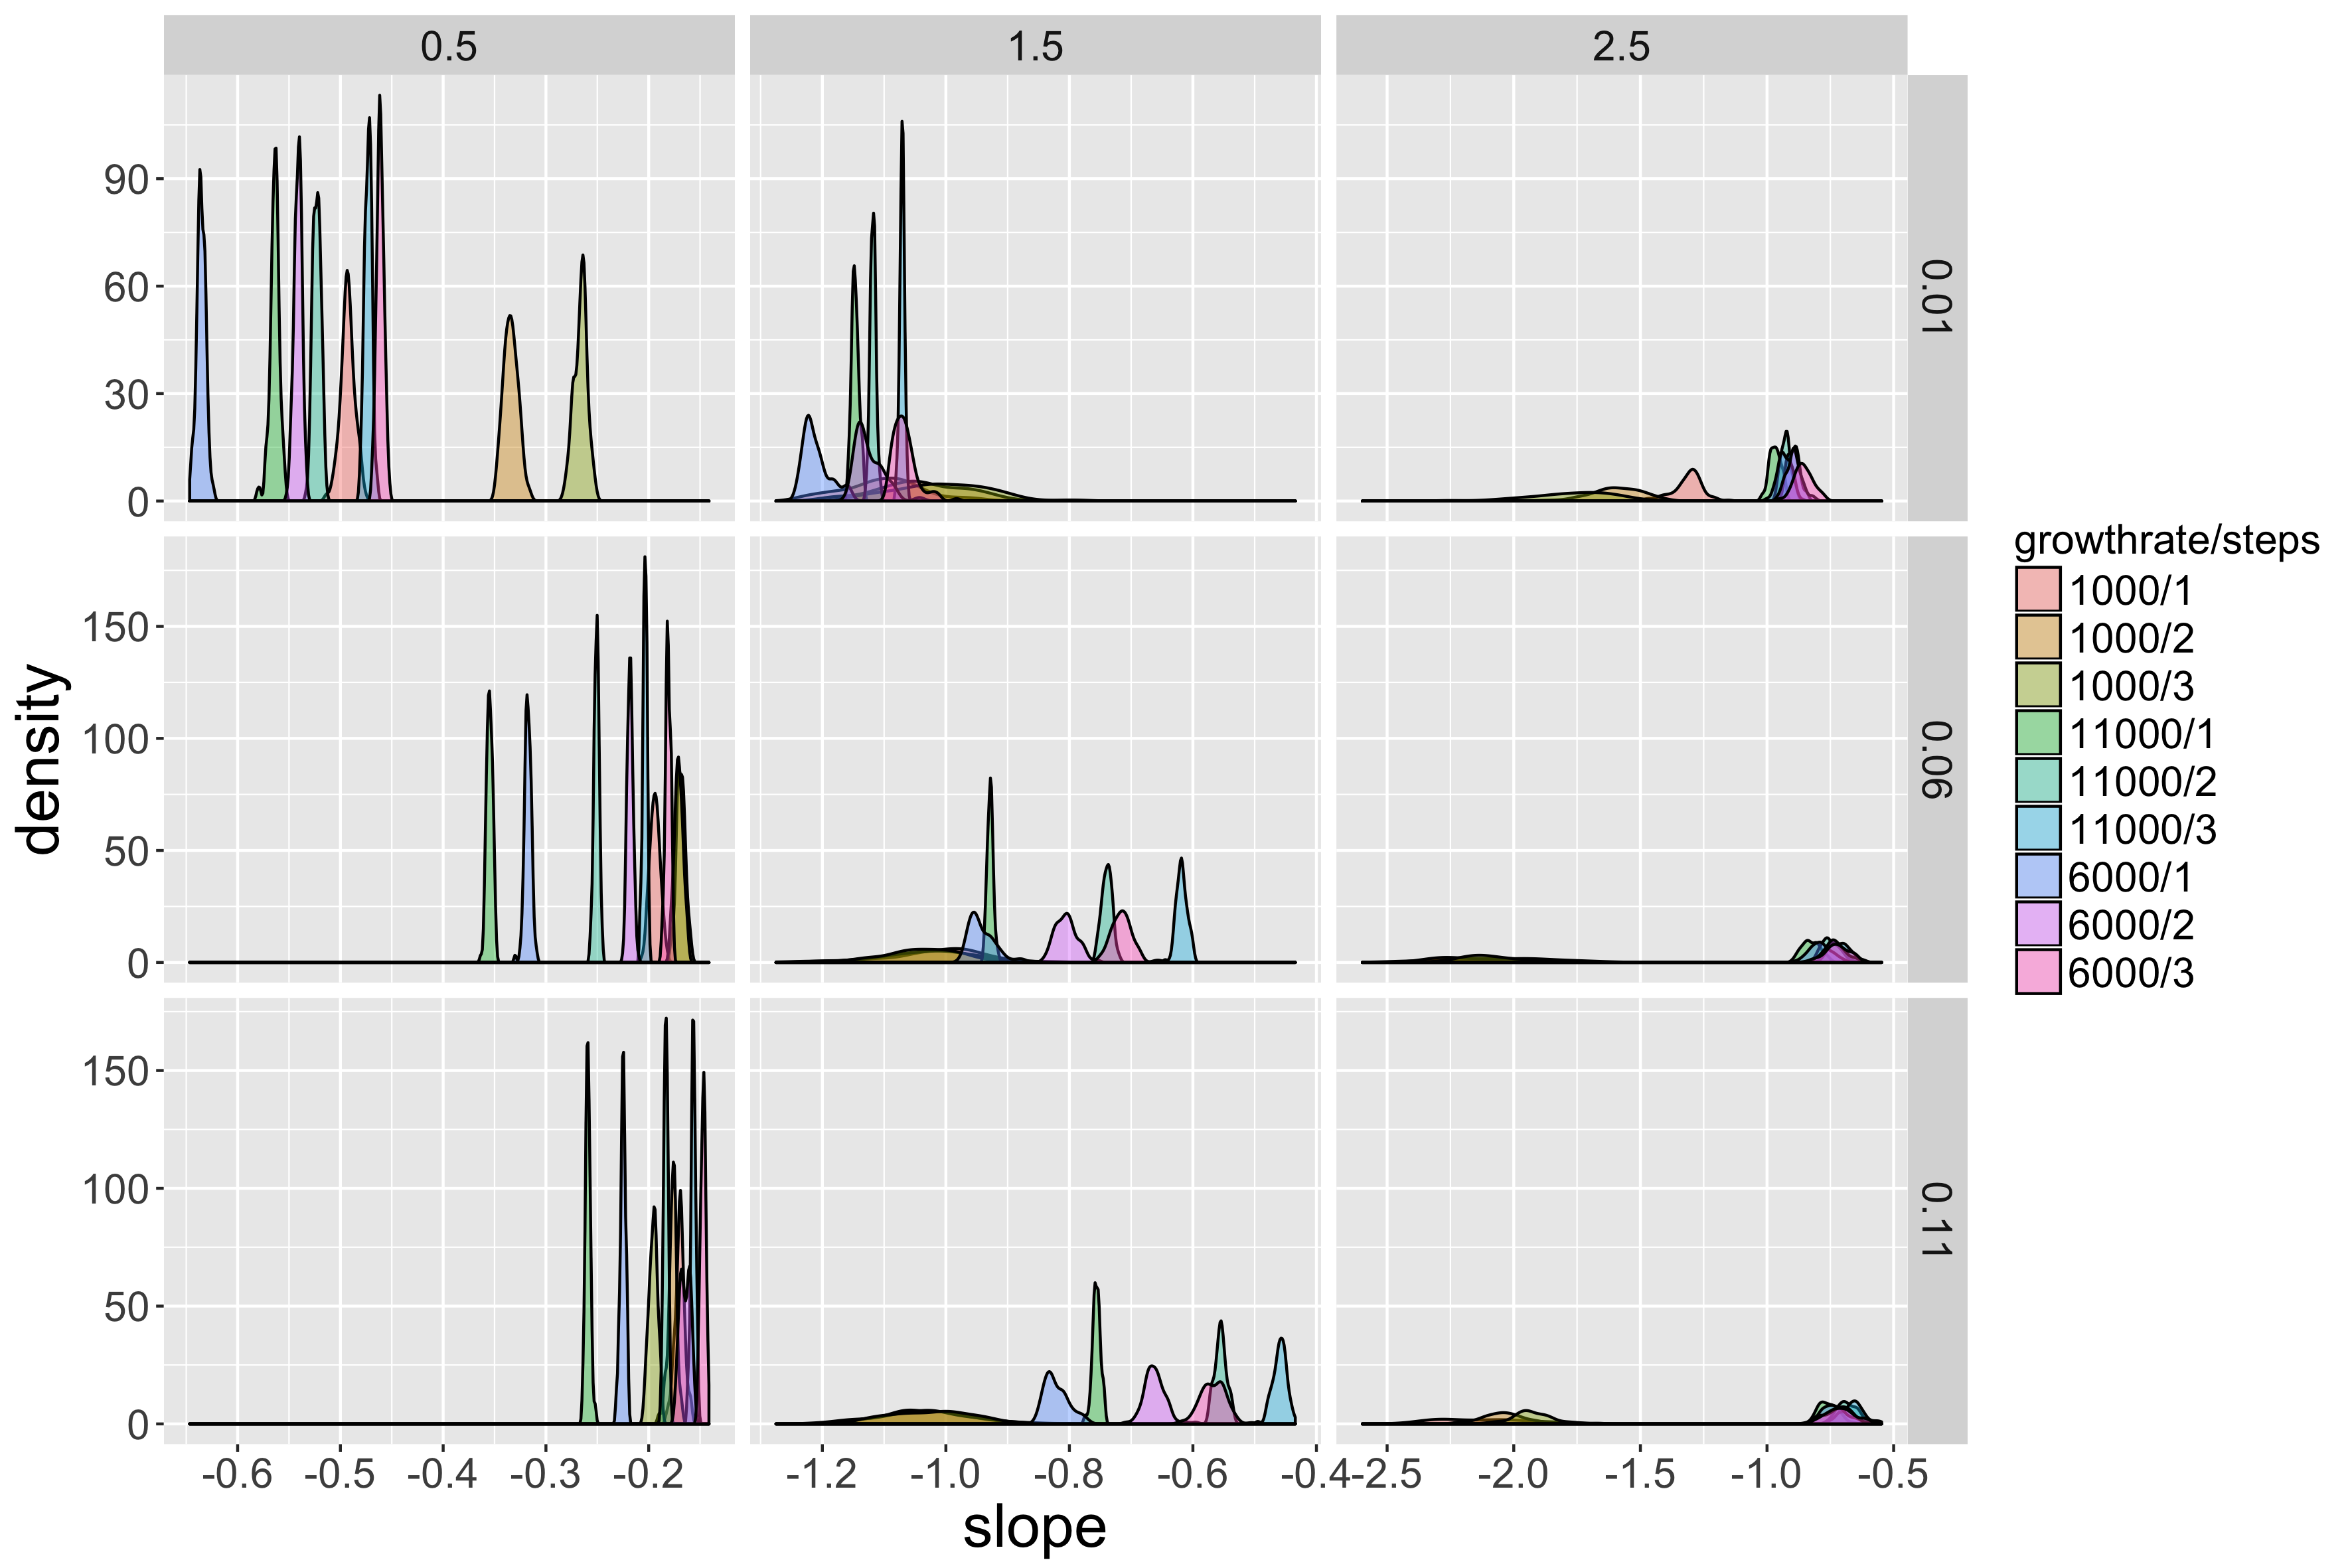
\includegraphics[width=0.8\textwidth]{Figures/Density/hist_slope}
\caption[][]{Histograms for Moran index (top) and slope (bottom), for varying $\alpha$ (columns), $\beta$ (rows), $N_G$ and $n_d$ (colors).}{}
\label{fig:histograms}
\end{figure}
%%%%%%%%%%%%%%%%%%%%






\subsubsection{Indicators Behavior}{Indicateurs}

% full plots behavior

We show in Fig. to Fig. 10 the full behavior of all indicators, with all parameters varying, obtained through the extensive exploration, from which the plots in main text have been extracted. Because of the complex nature of emergent urban form, one can not predict output values without referring to this ``exhaustive'' parameter sweep.


%%%%%%%%%%%%%%%%%%%%
\begin{figure}
\centering
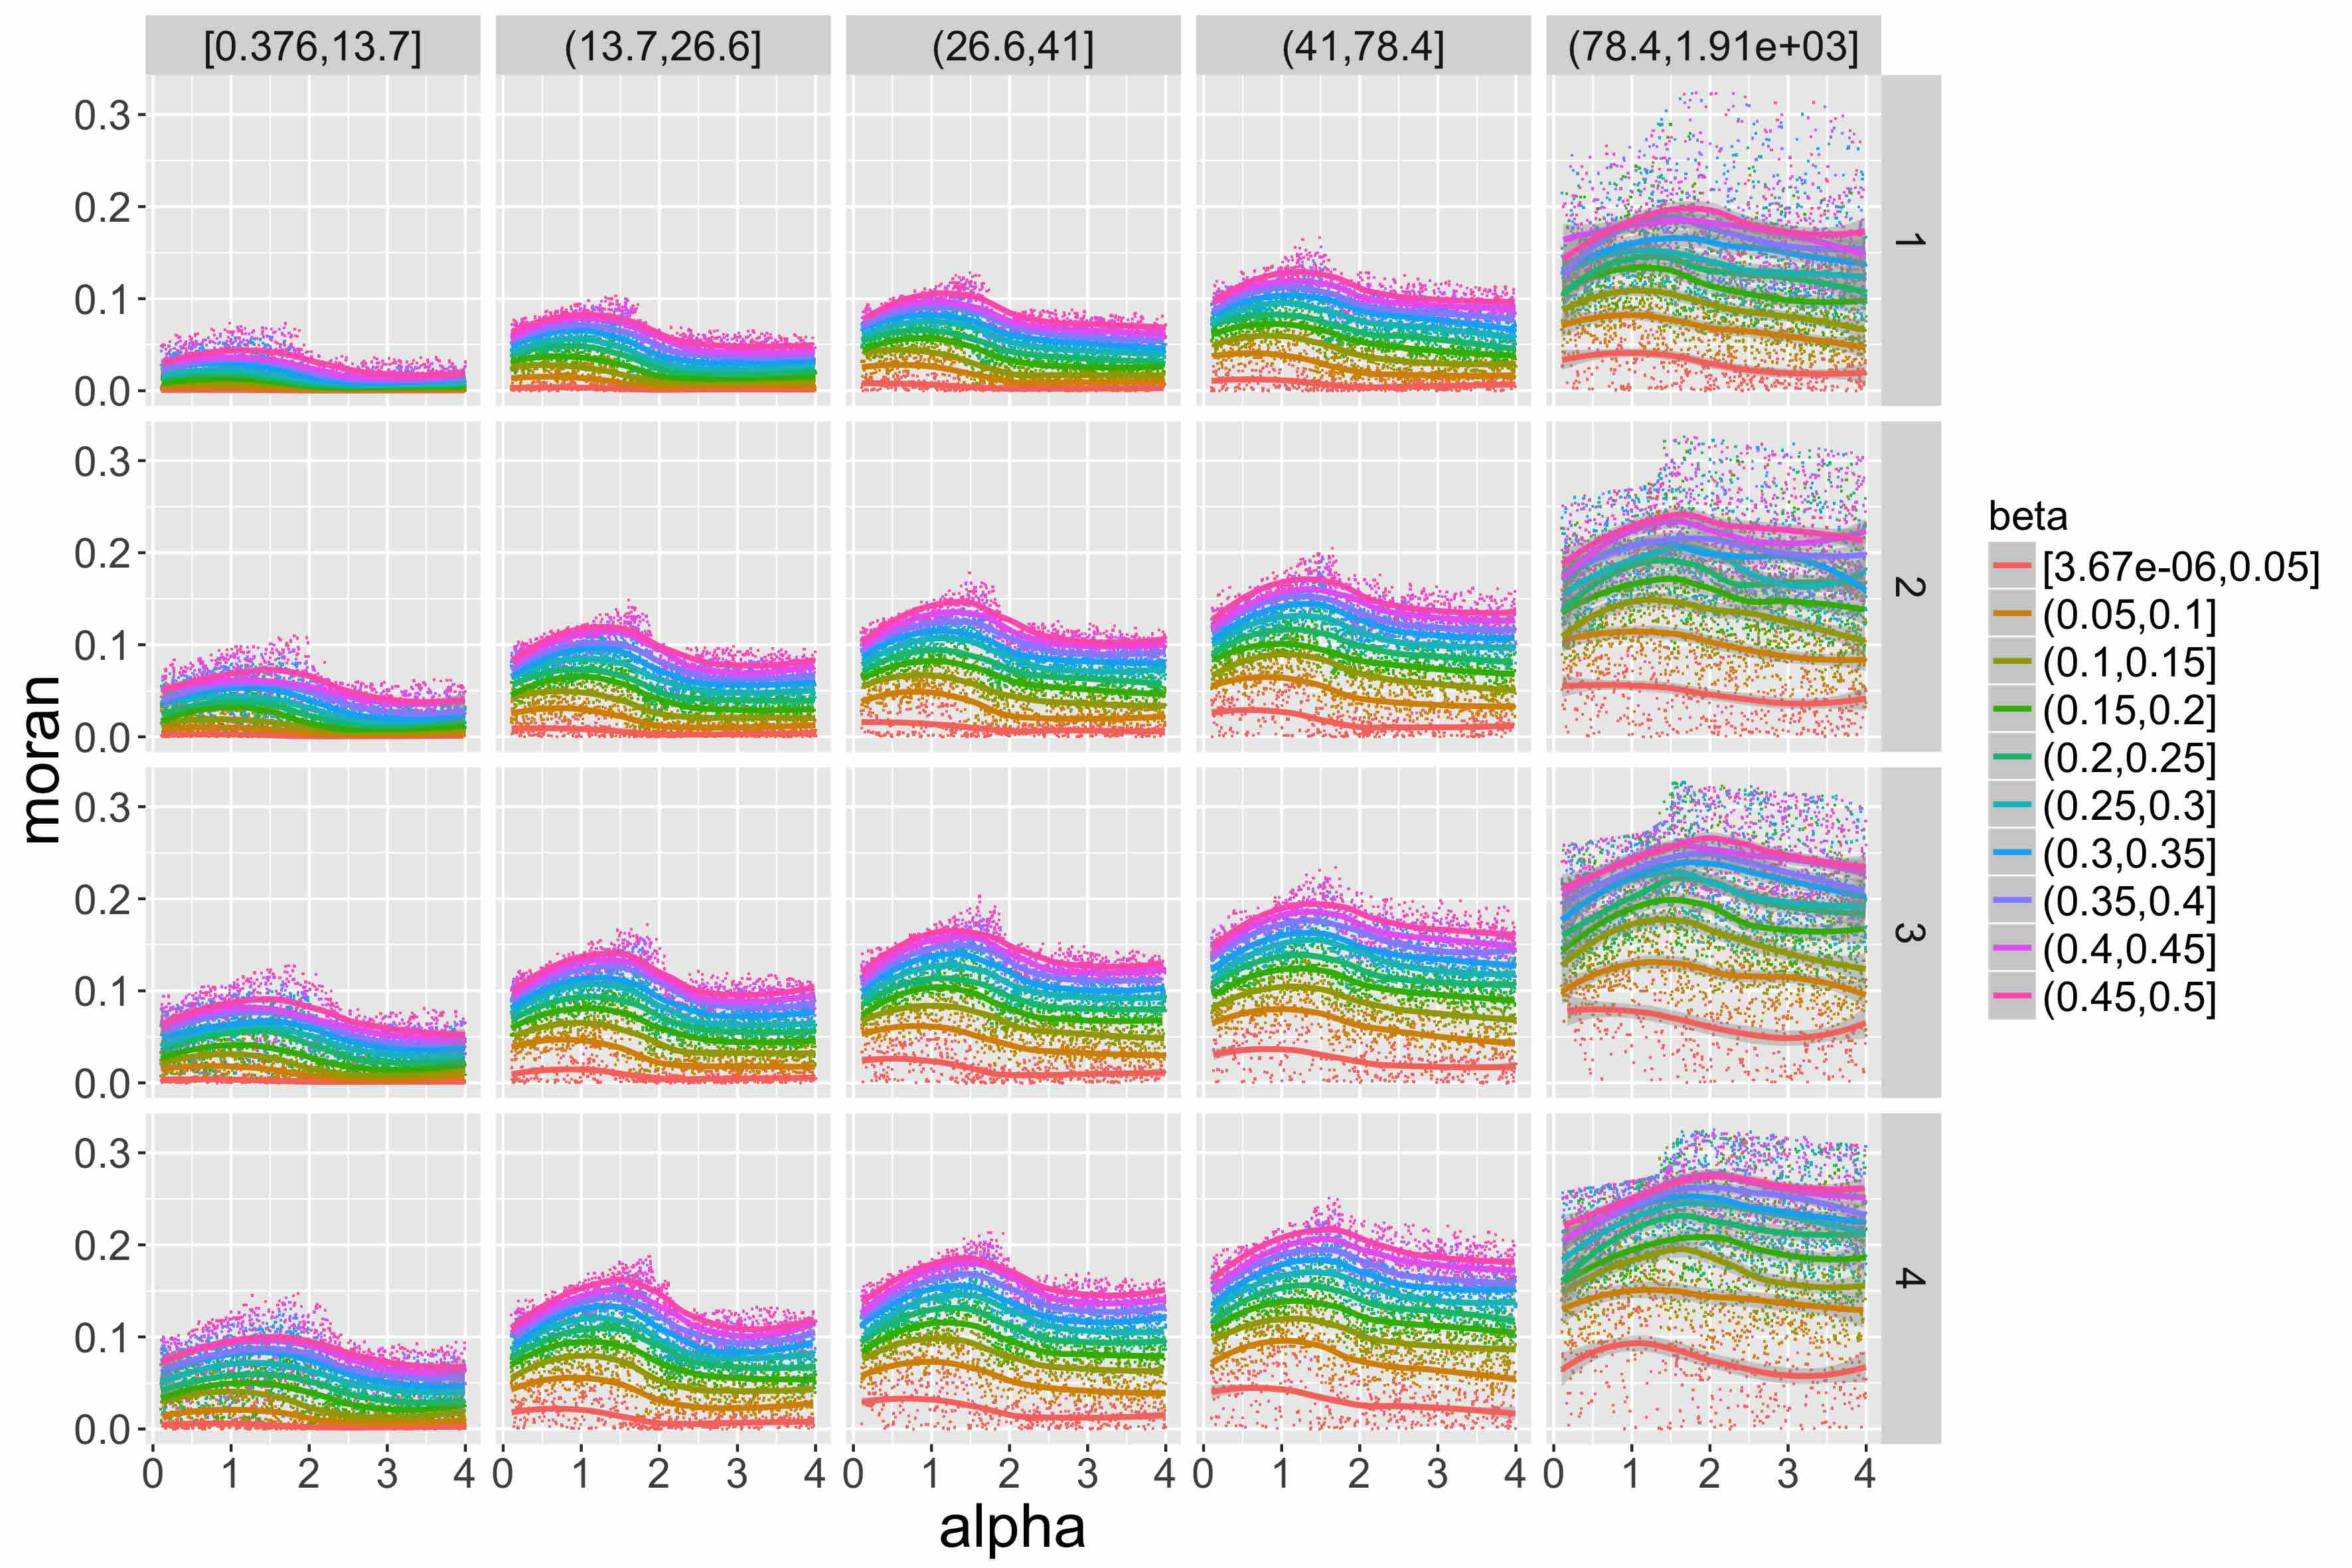
\includegraphics[width=0.8\textwidth]{Figures/Density/moran_alpha}
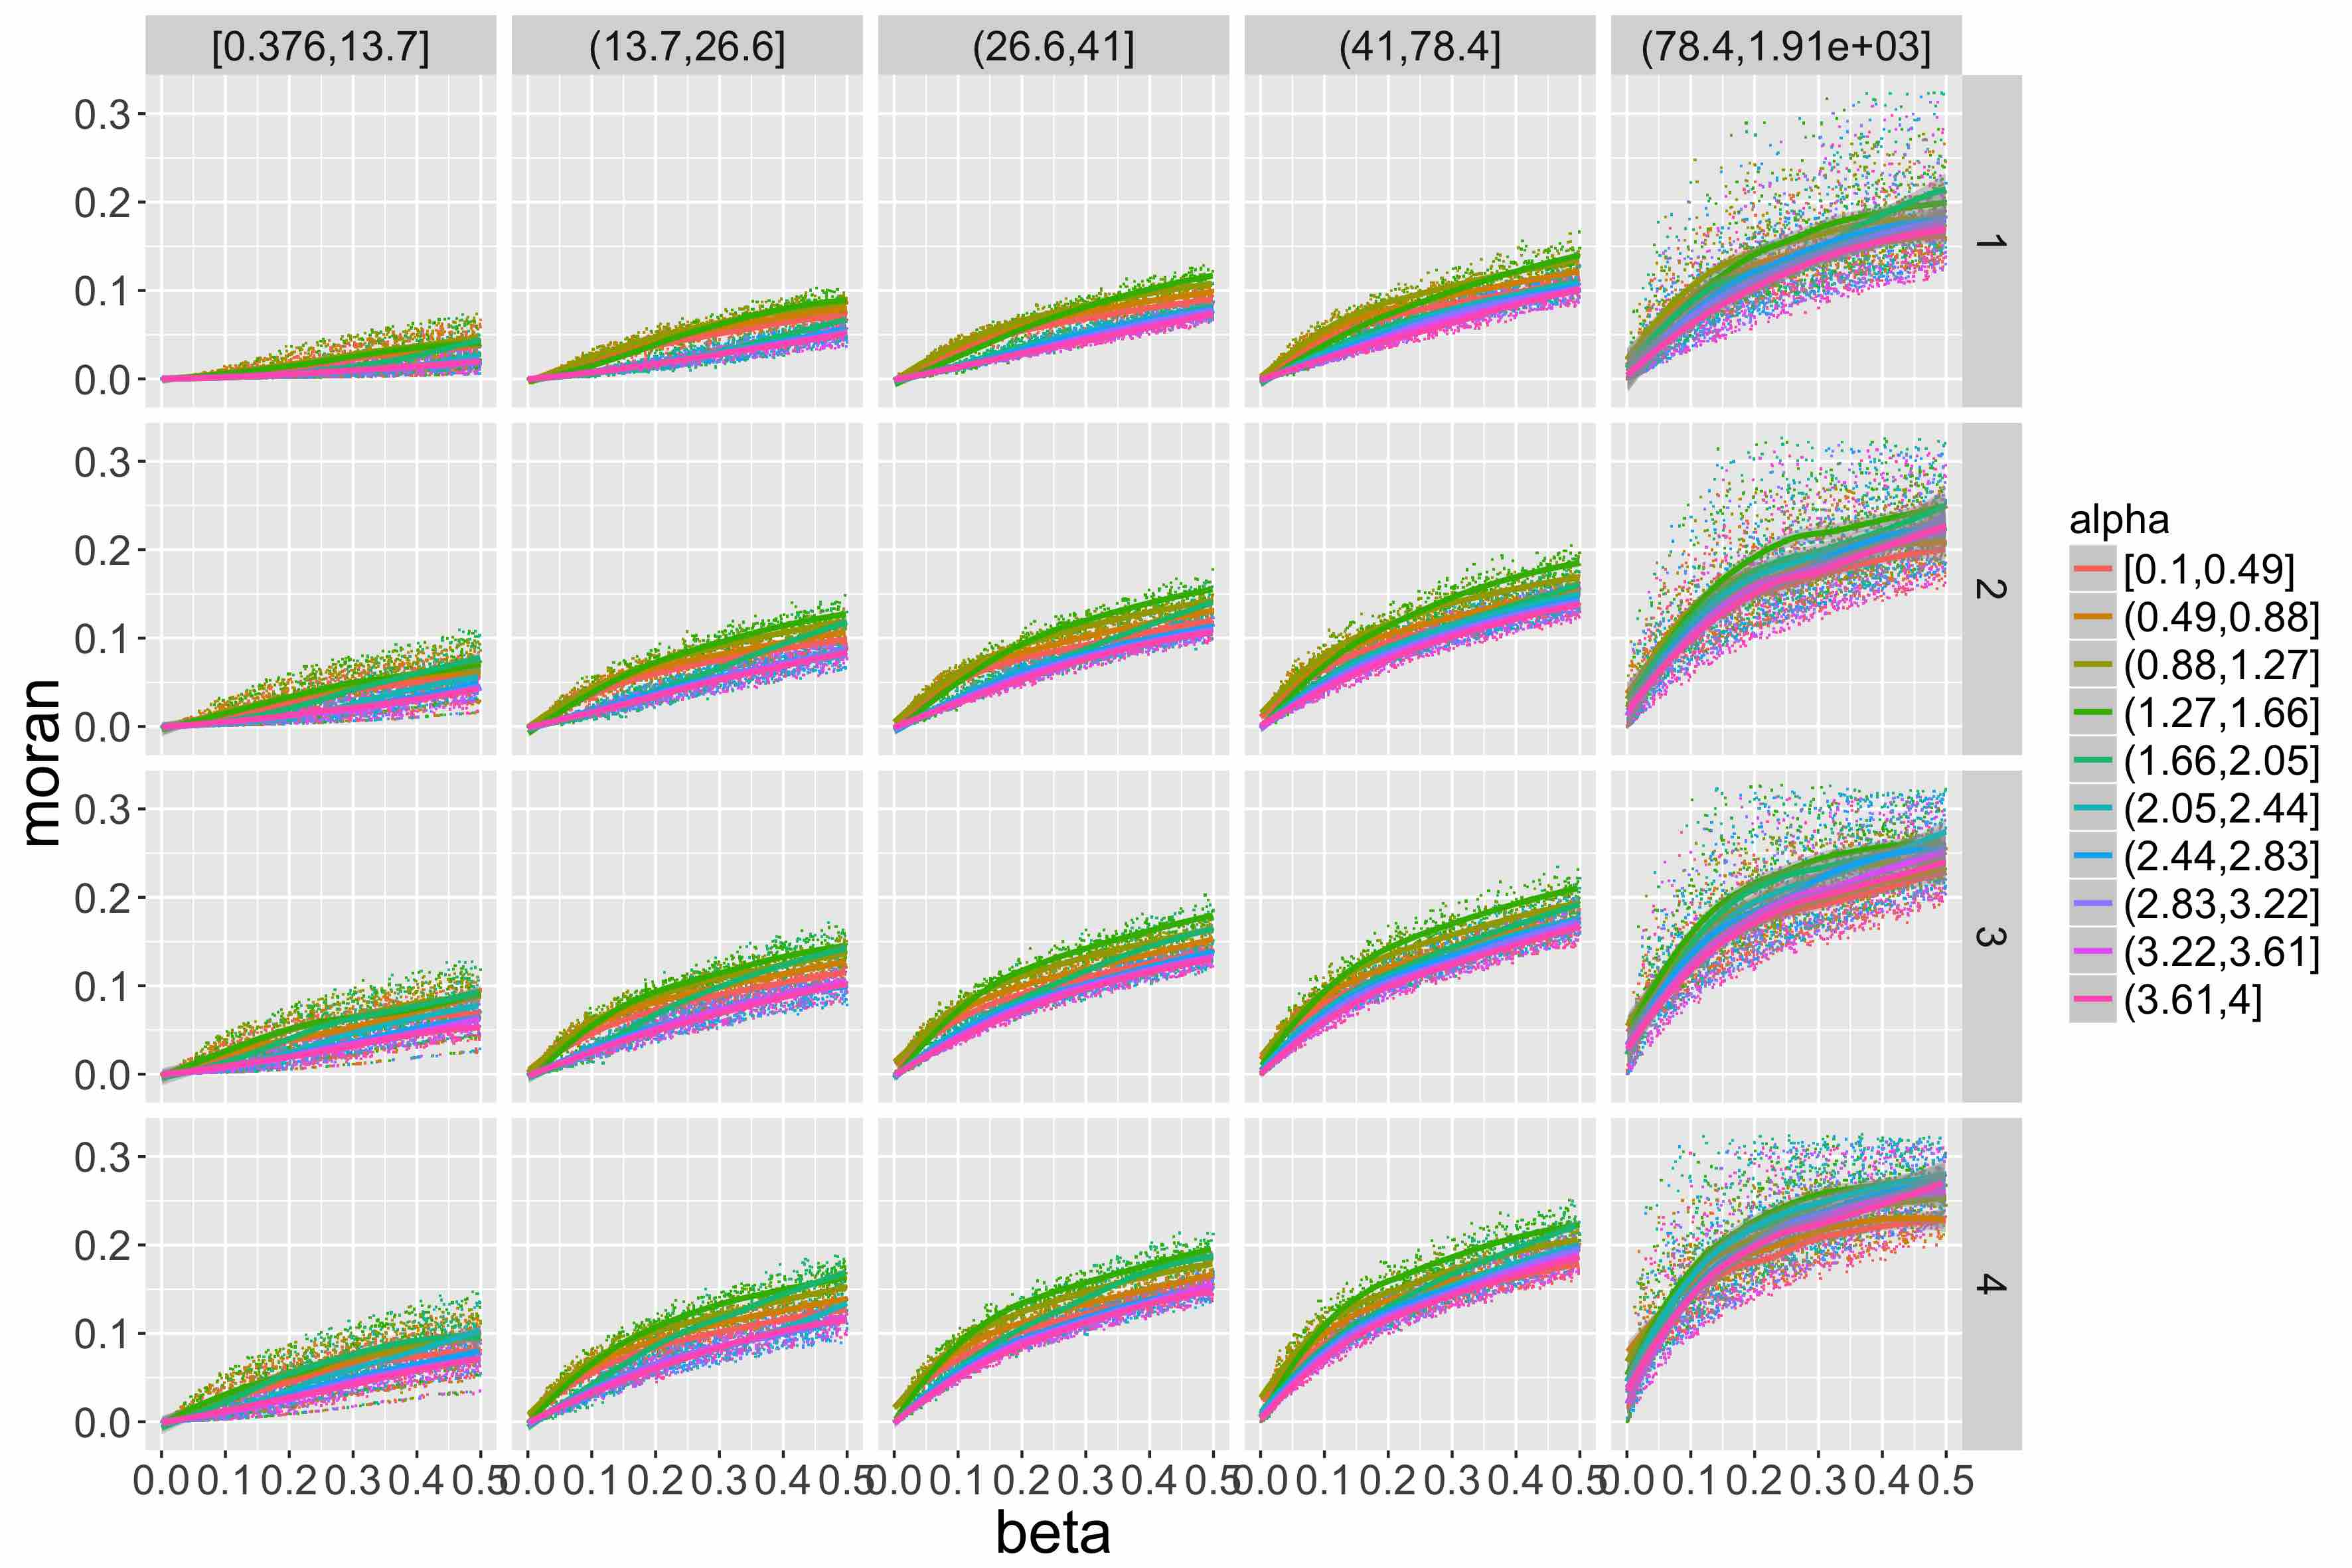
\includegraphics[width=0.8\textwidth]{Figures/Density/moran_beta}
\caption[][]{Moran index as a function of $\alpha$ (Top) and $\beta$ (Bottom) for varying $\beta$ (resp. $\alpha$) given by color, and varying $n_d$ (rows) and $N_G$ (columns).}{}
\label{fig:moran}
\end{figure}
%%%%%%%%%%%%%%%%%%%%

%%%%%%%%%%%%%%%%%%%%
\begin{figure}
\centering
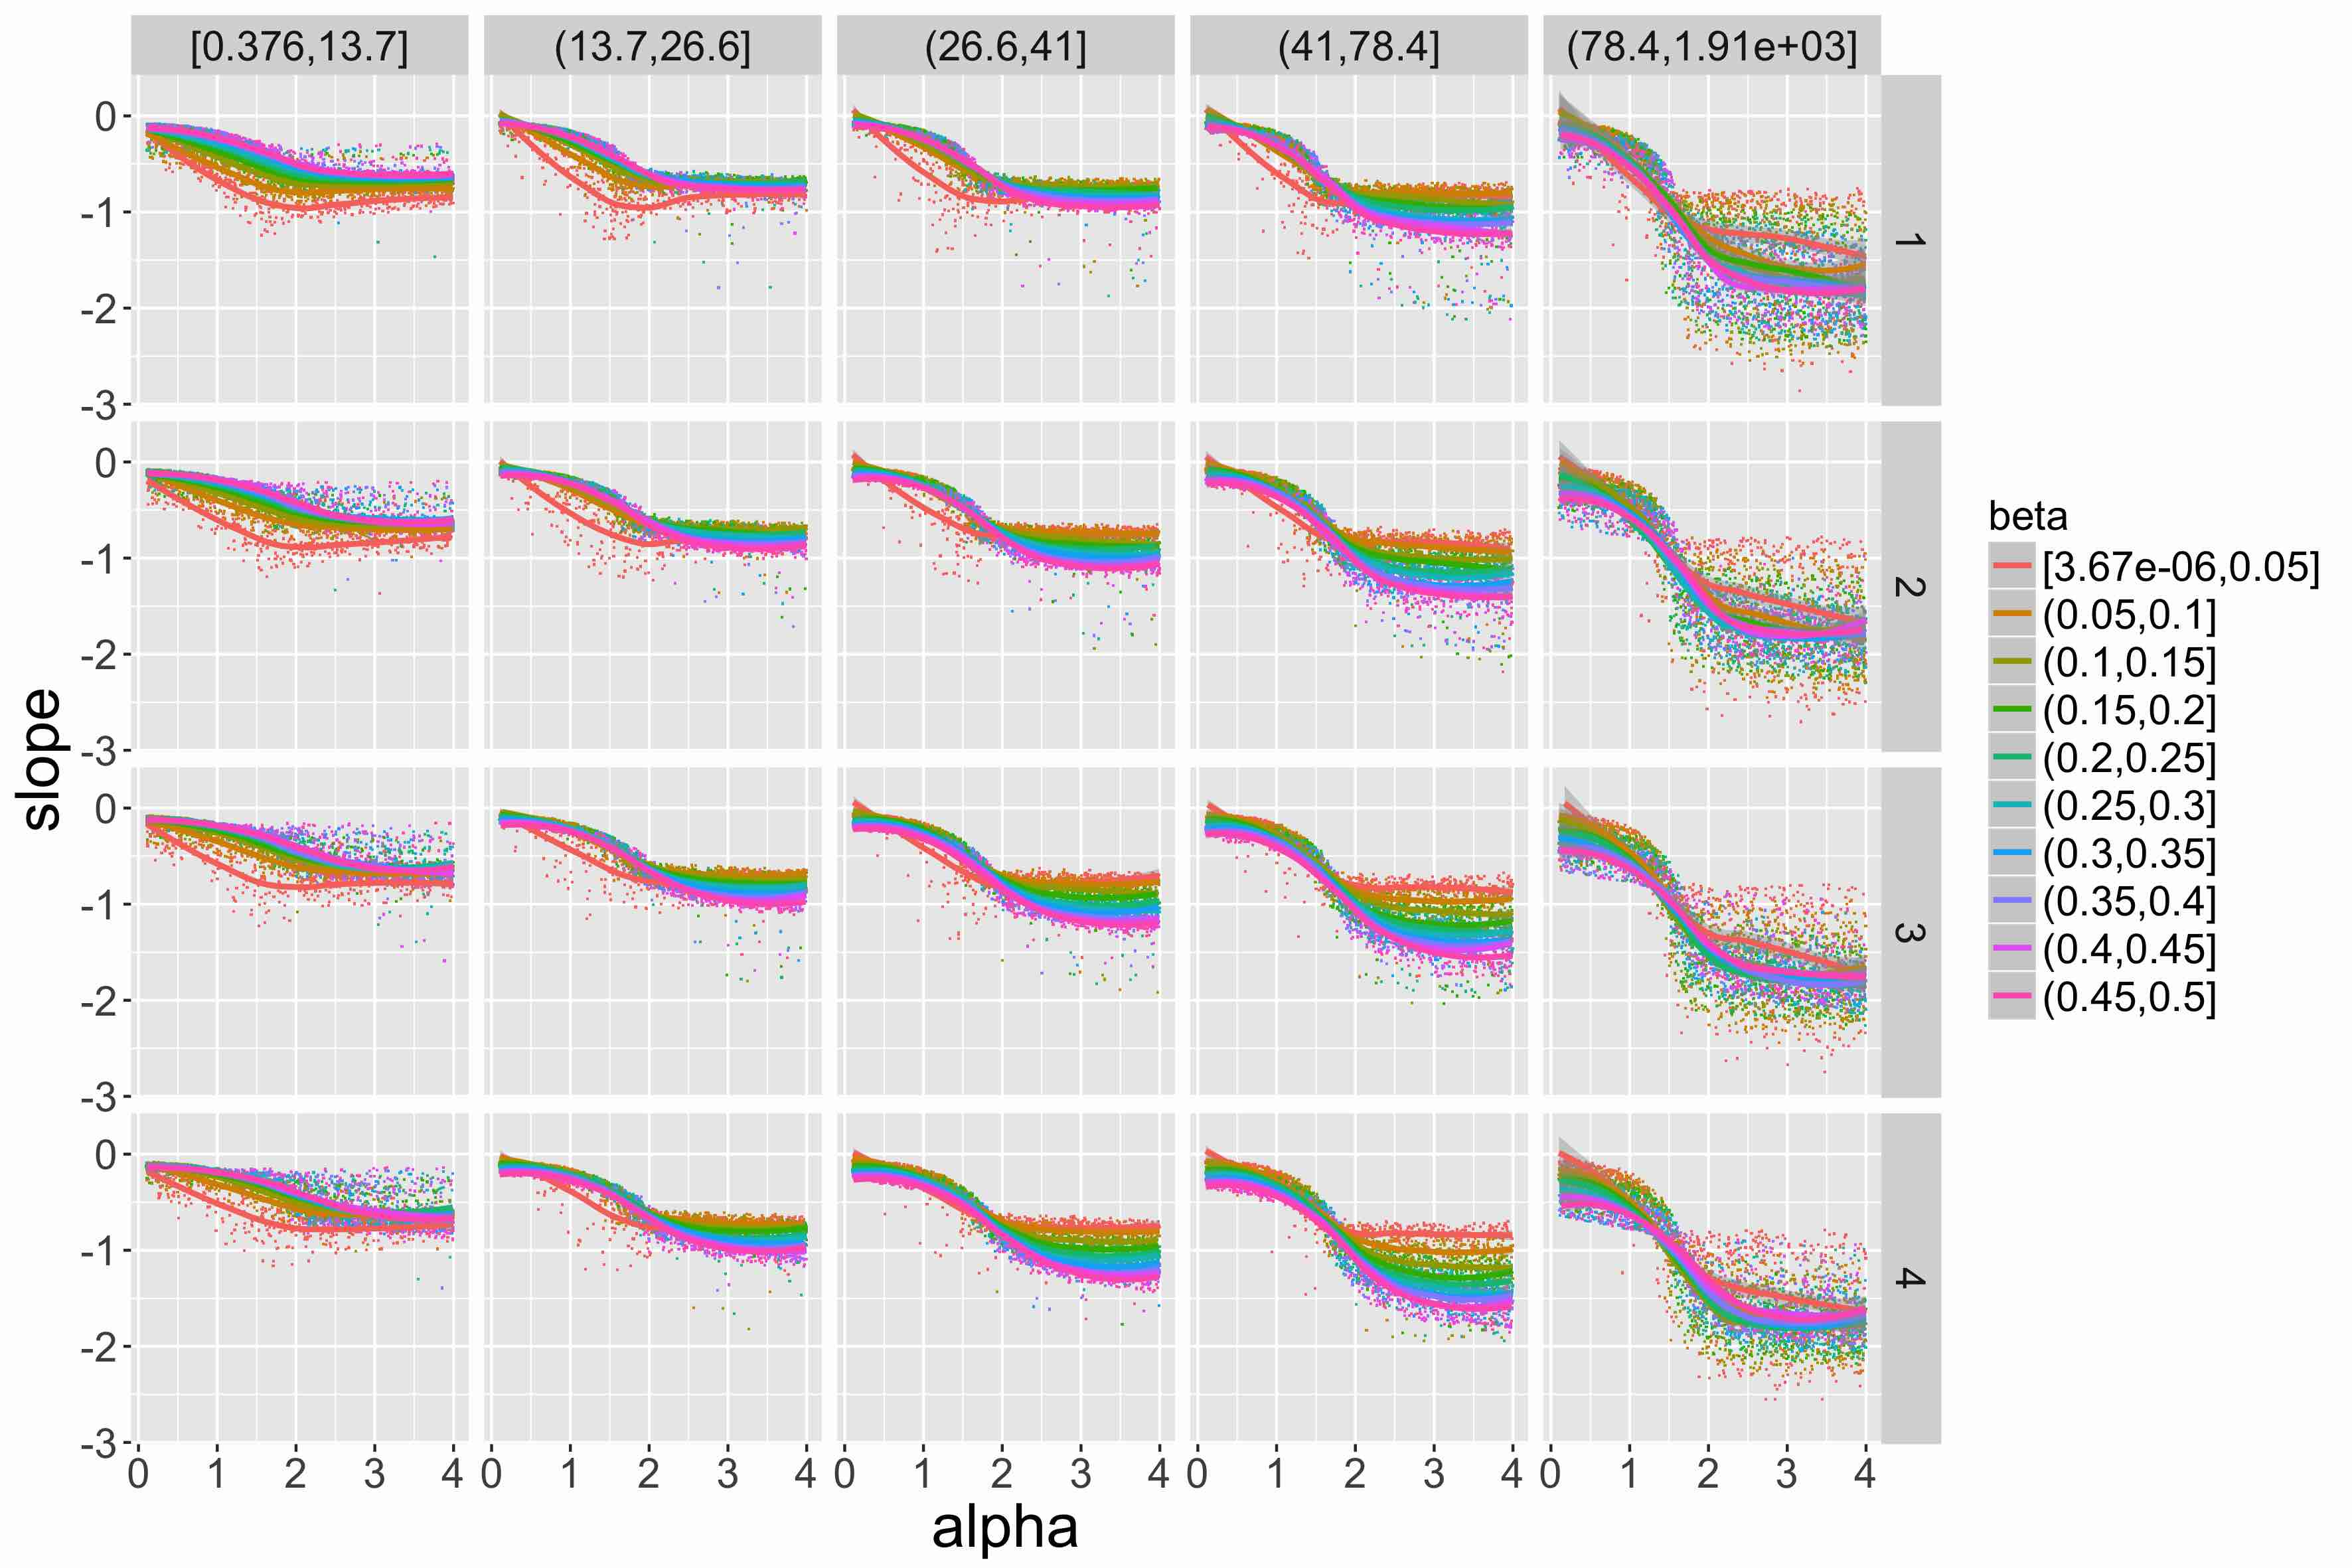
\includegraphics[width=0.8\textwidth]{Figures/Density/slope_alpha}
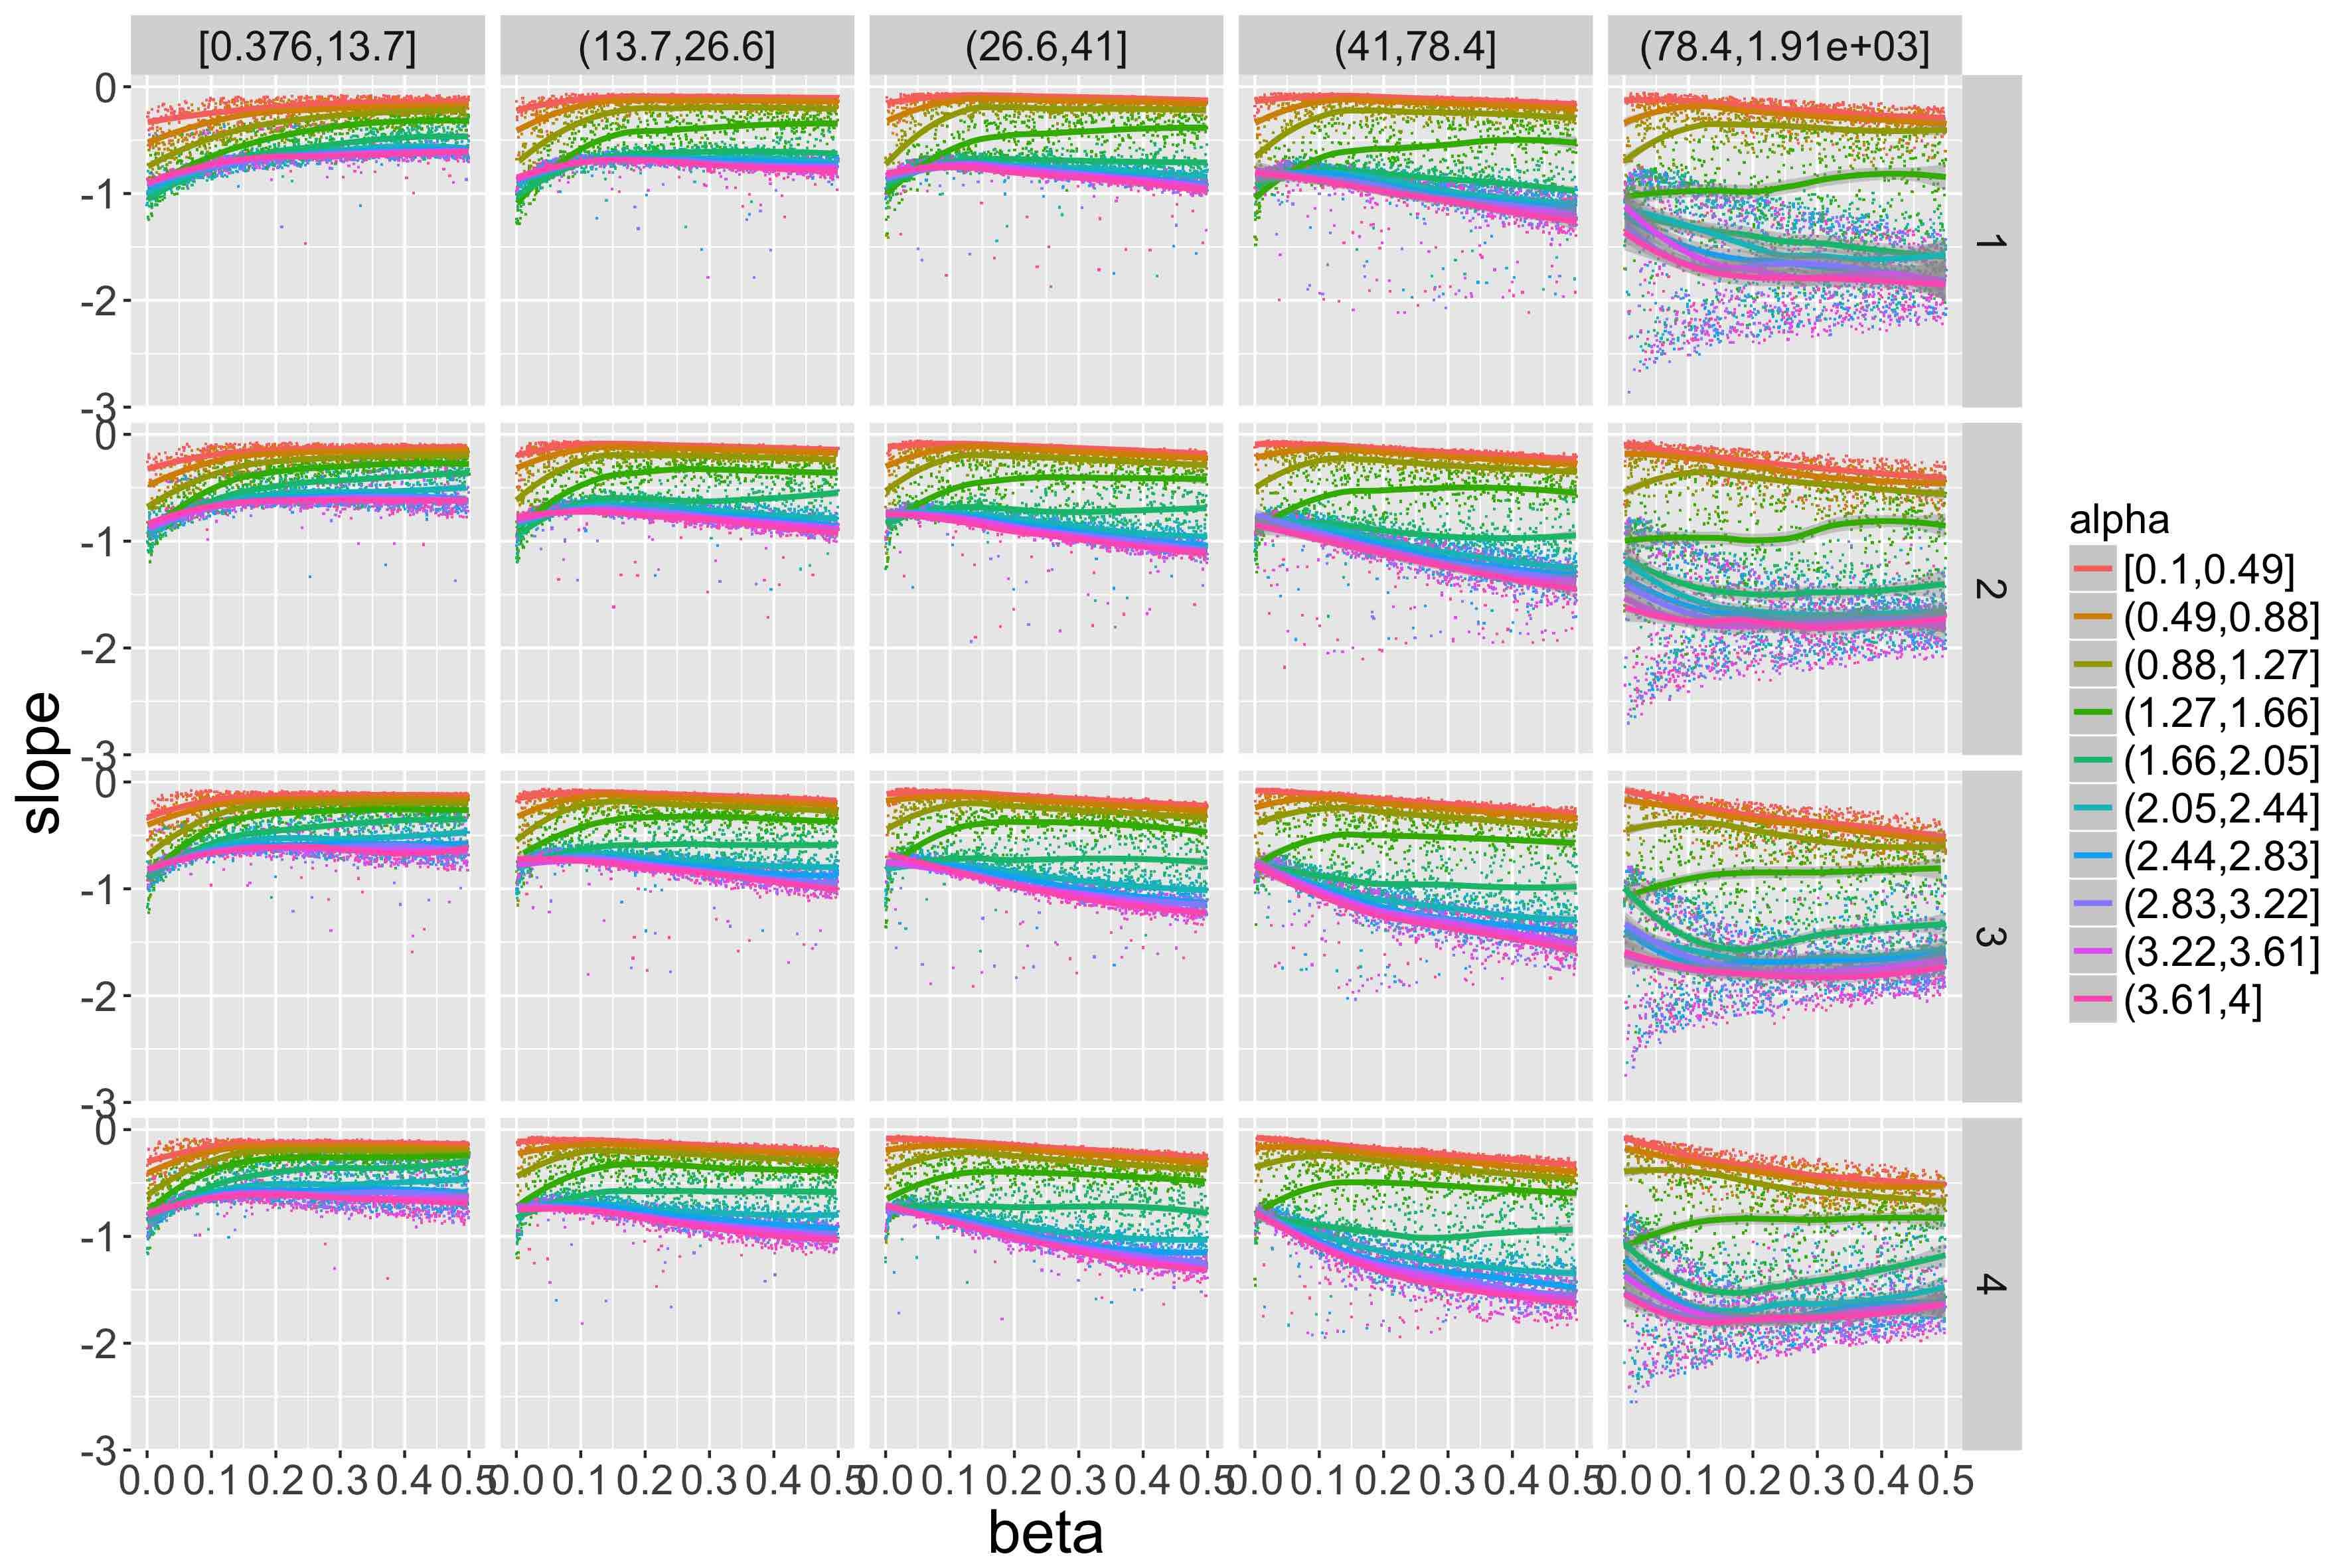
\includegraphics[width=0.8\textwidth]{Figures/Density/slope_beta}
\caption[][]{Slope as a function of $\alpha$ (Top) and $\beta$ (Bottom) for varying $\beta$ (resp. $\alpha$) given by color, and varying $n_d$ (rows) and $N_G$ (columns).}{}
\label{fig:slope}
\end{figure}
%%%%%%%%%%%%%%%%%%%%


%%%%%%%%%%%%%%%%%%%%
\begin{figure}
\centering
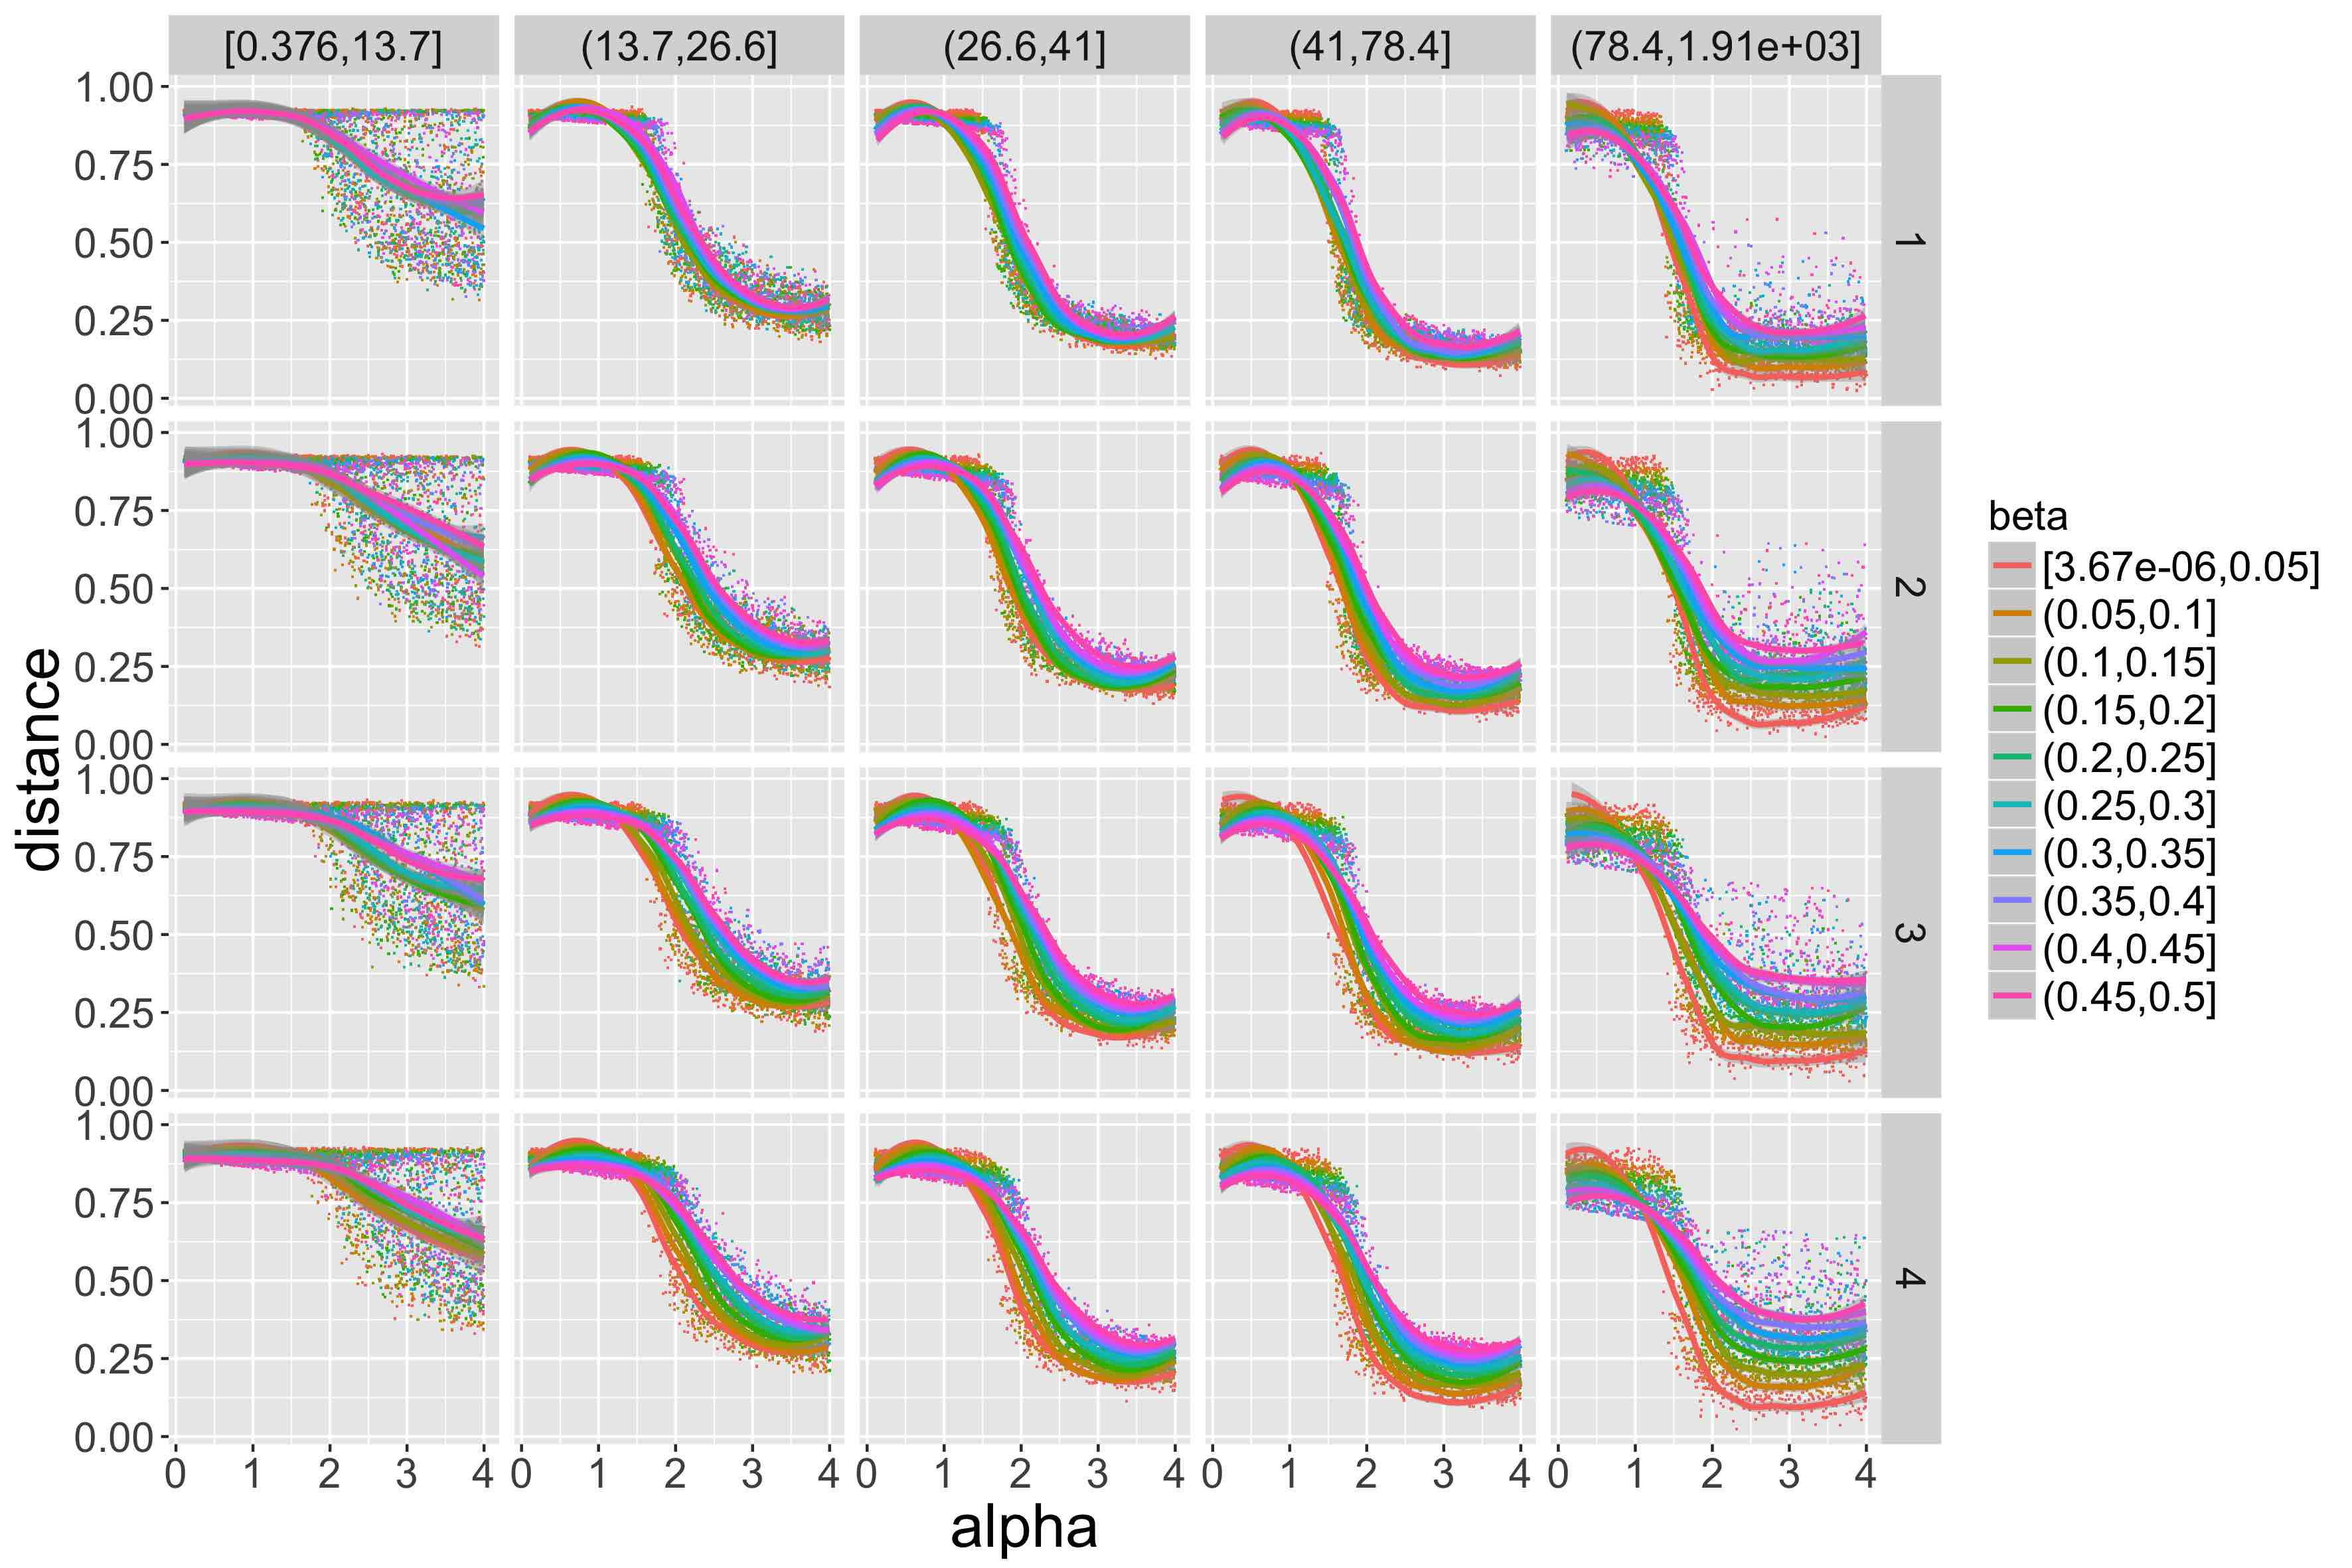
\includegraphics[width=0.8\textwidth]{Figures/Density/distance_alpha}
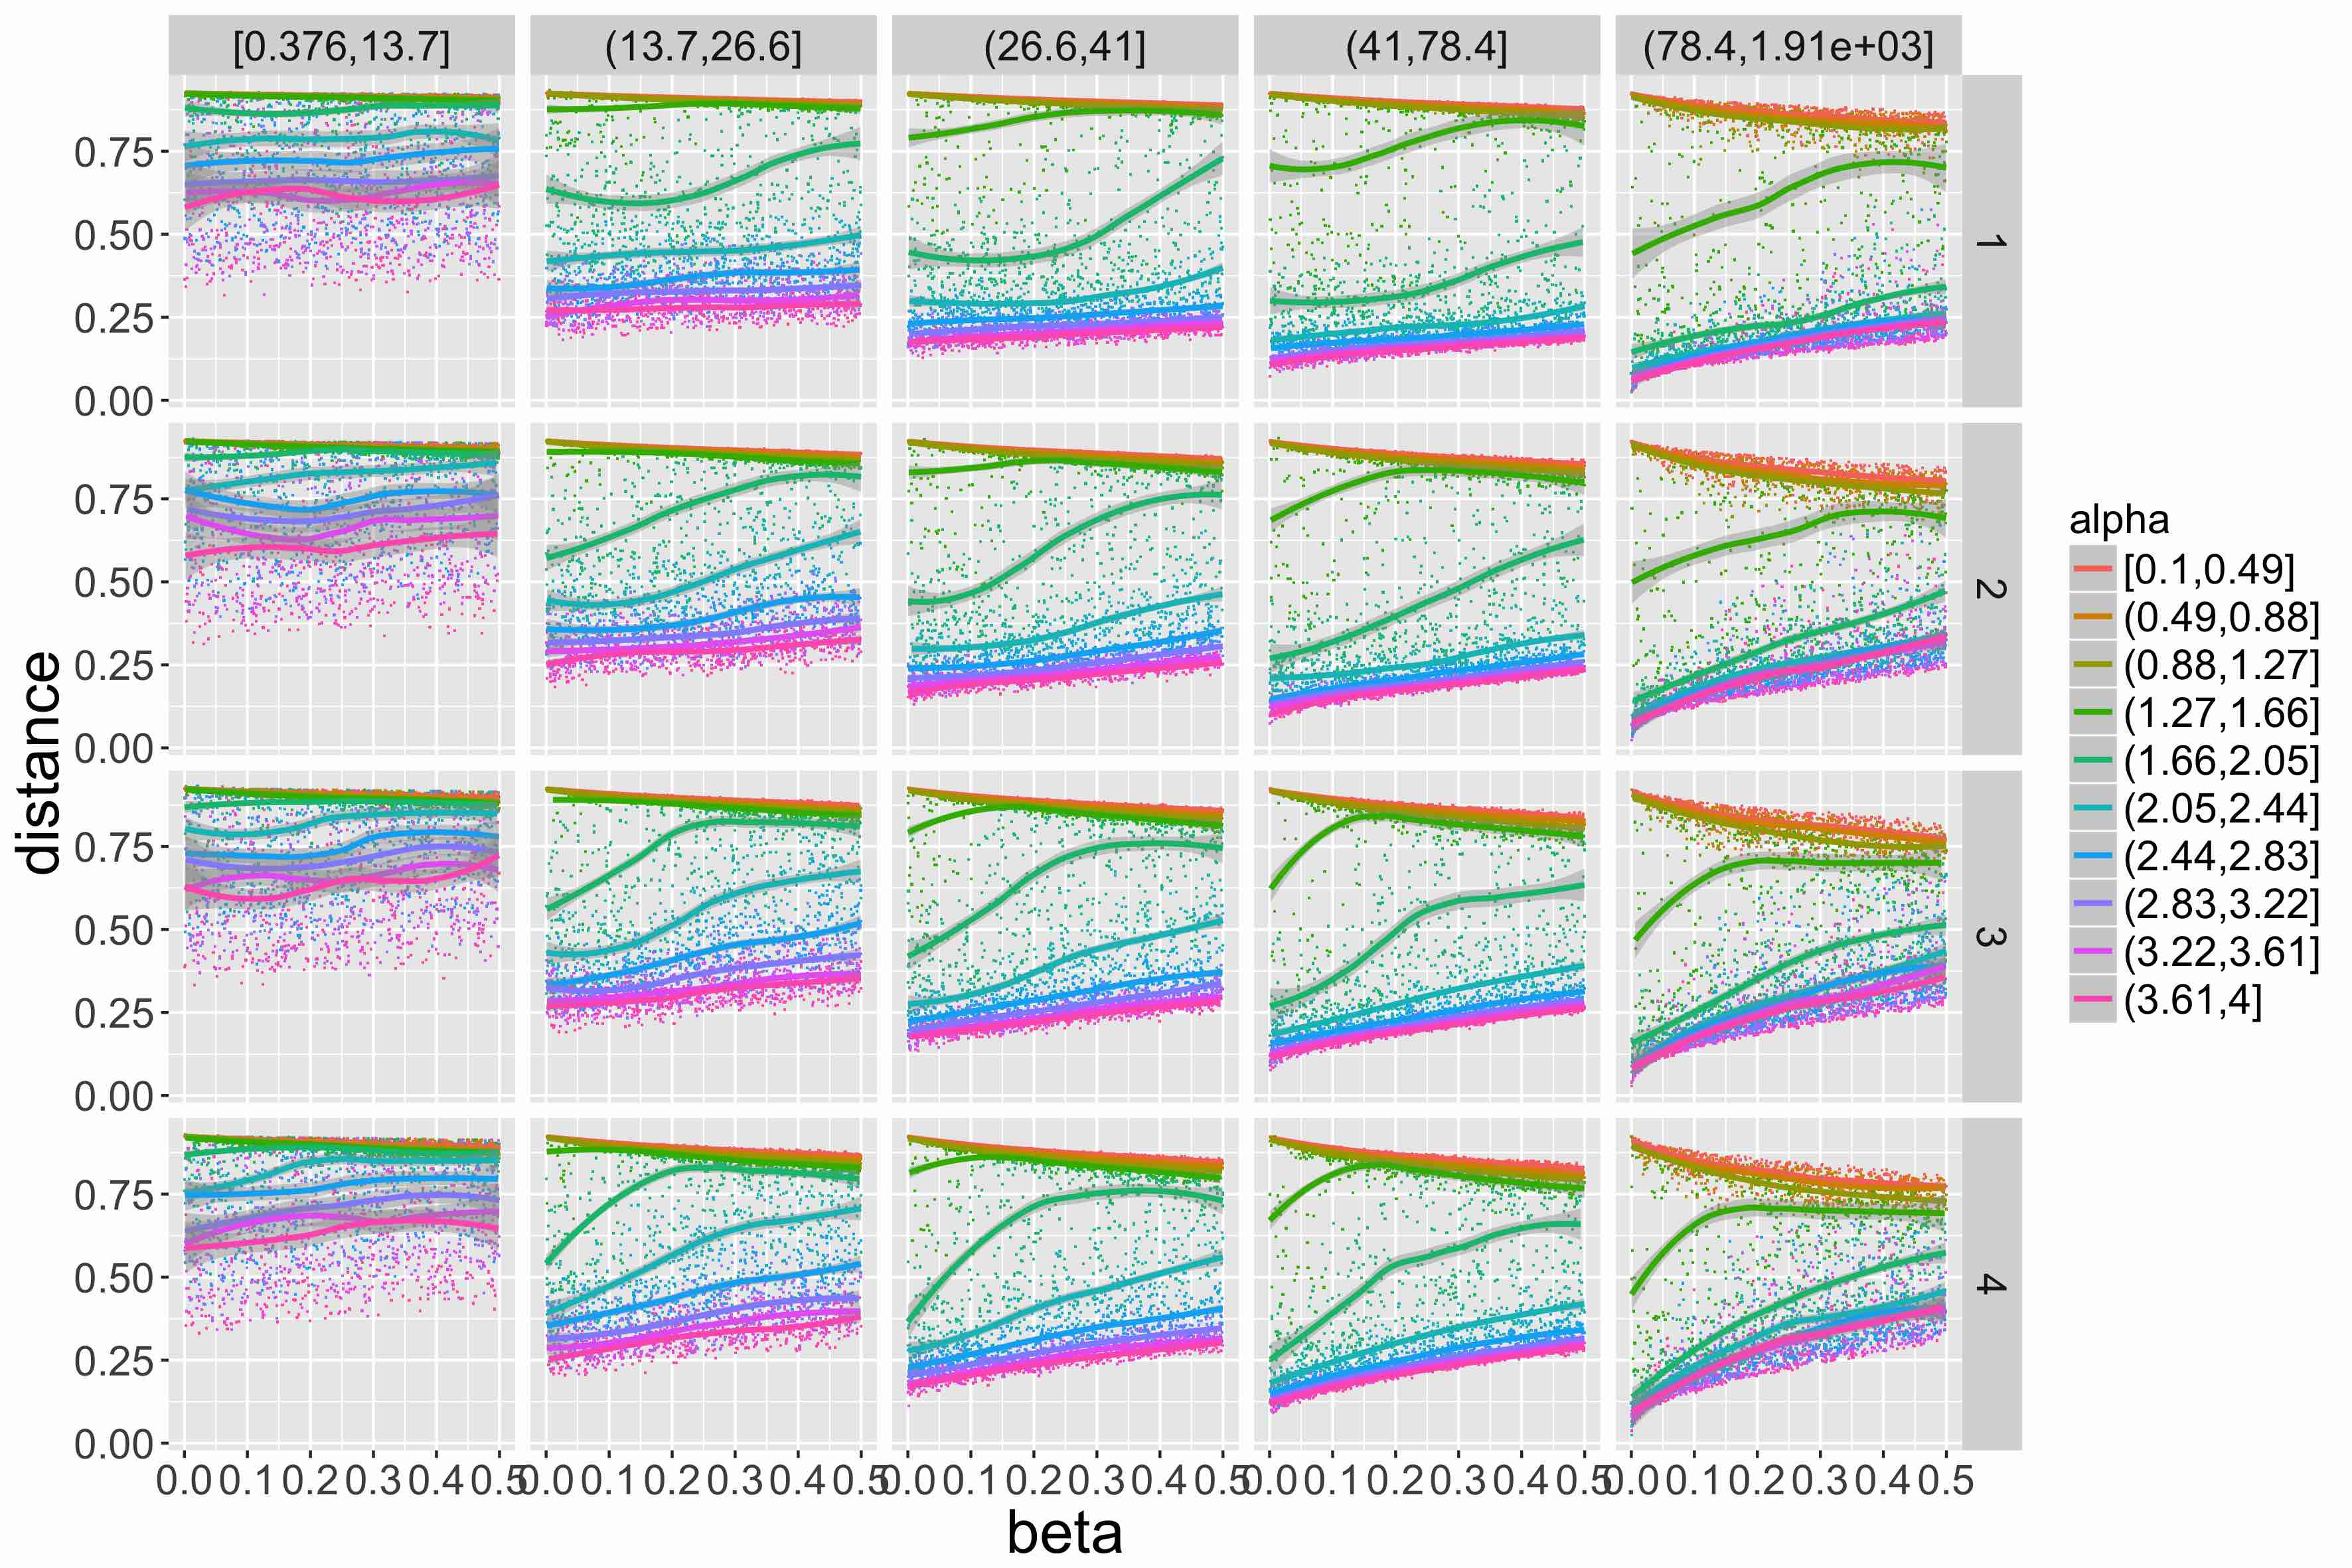
\includegraphics[width=0.8\textwidth]{Figures/Density/distance_beta}
\caption[][]{Average distance index as a function of $\alpha$ (Top) and $\beta$ (Bottom) for varying $\beta$ (resp. $\alpha$) given by color, and varying $n_d$ (rows) and $N_G$ (columns).}{}
\label{}
\end{figure}
%%%%%%%%%%%%%%%%%%%%

%%%%%%%%%%%%%%%%%%%%
\begin{figure}
\centering
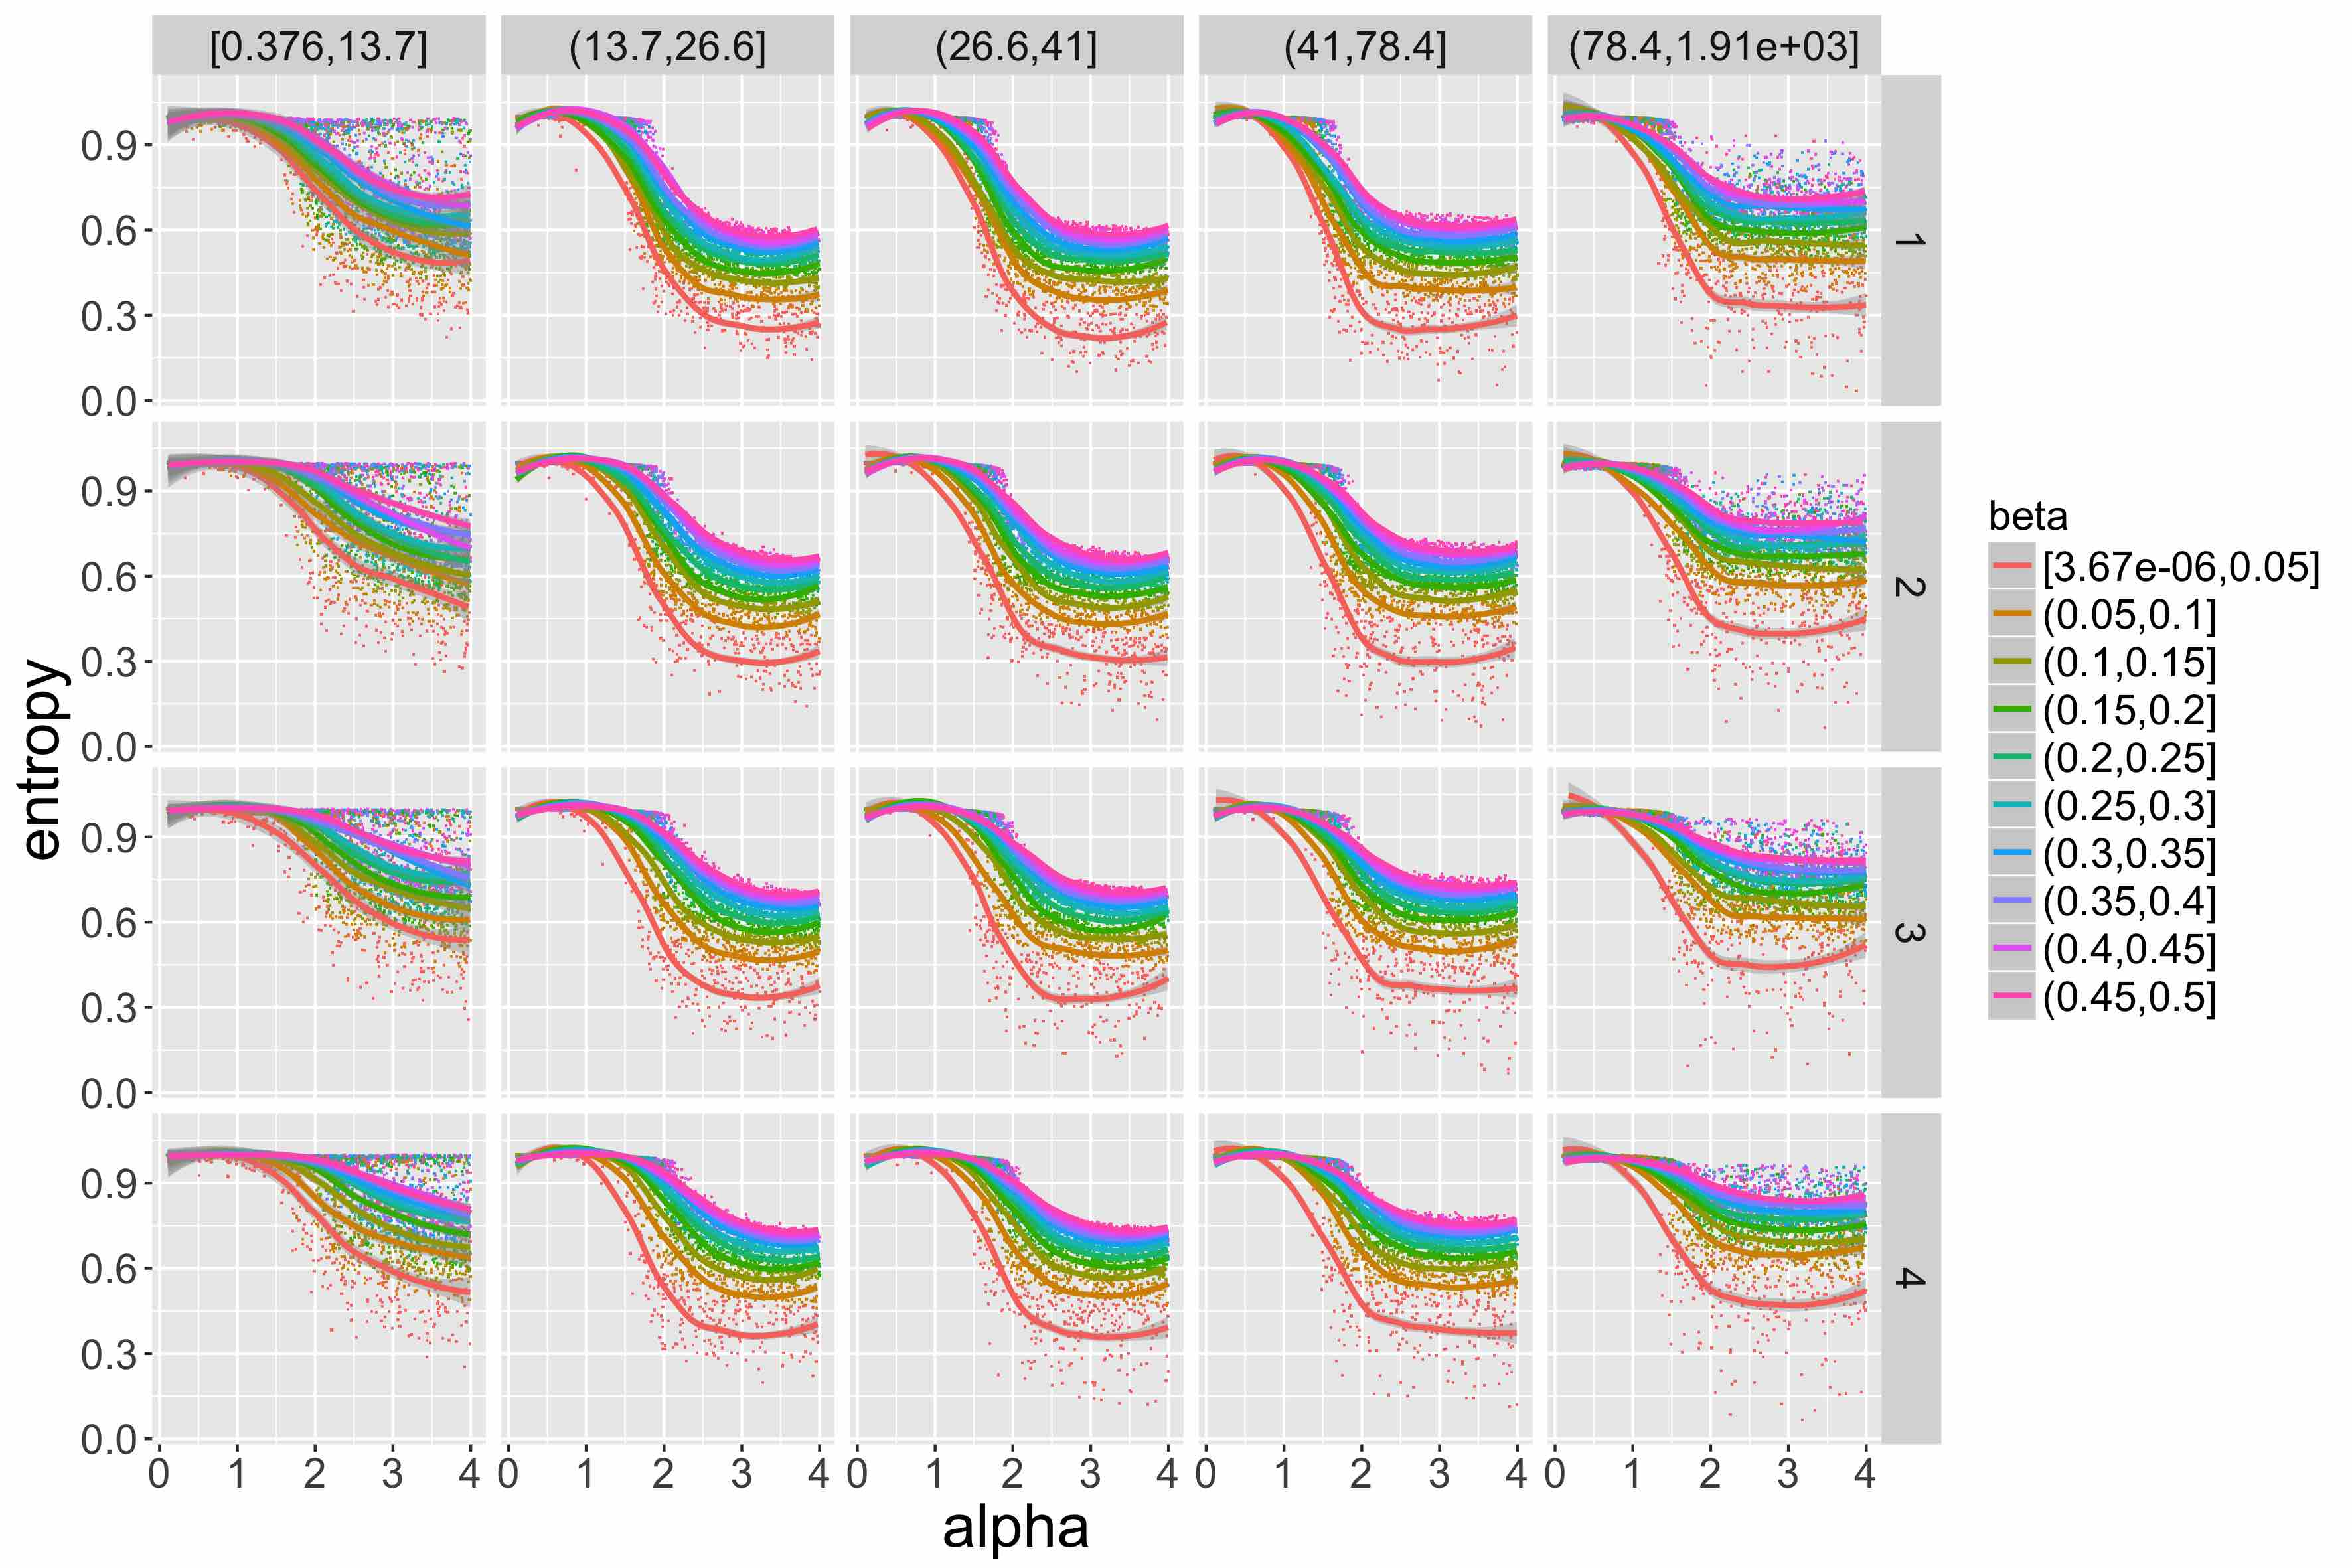
\includegraphics[width=0.8\textwidth]{Figures/Density/entropy_alpha}
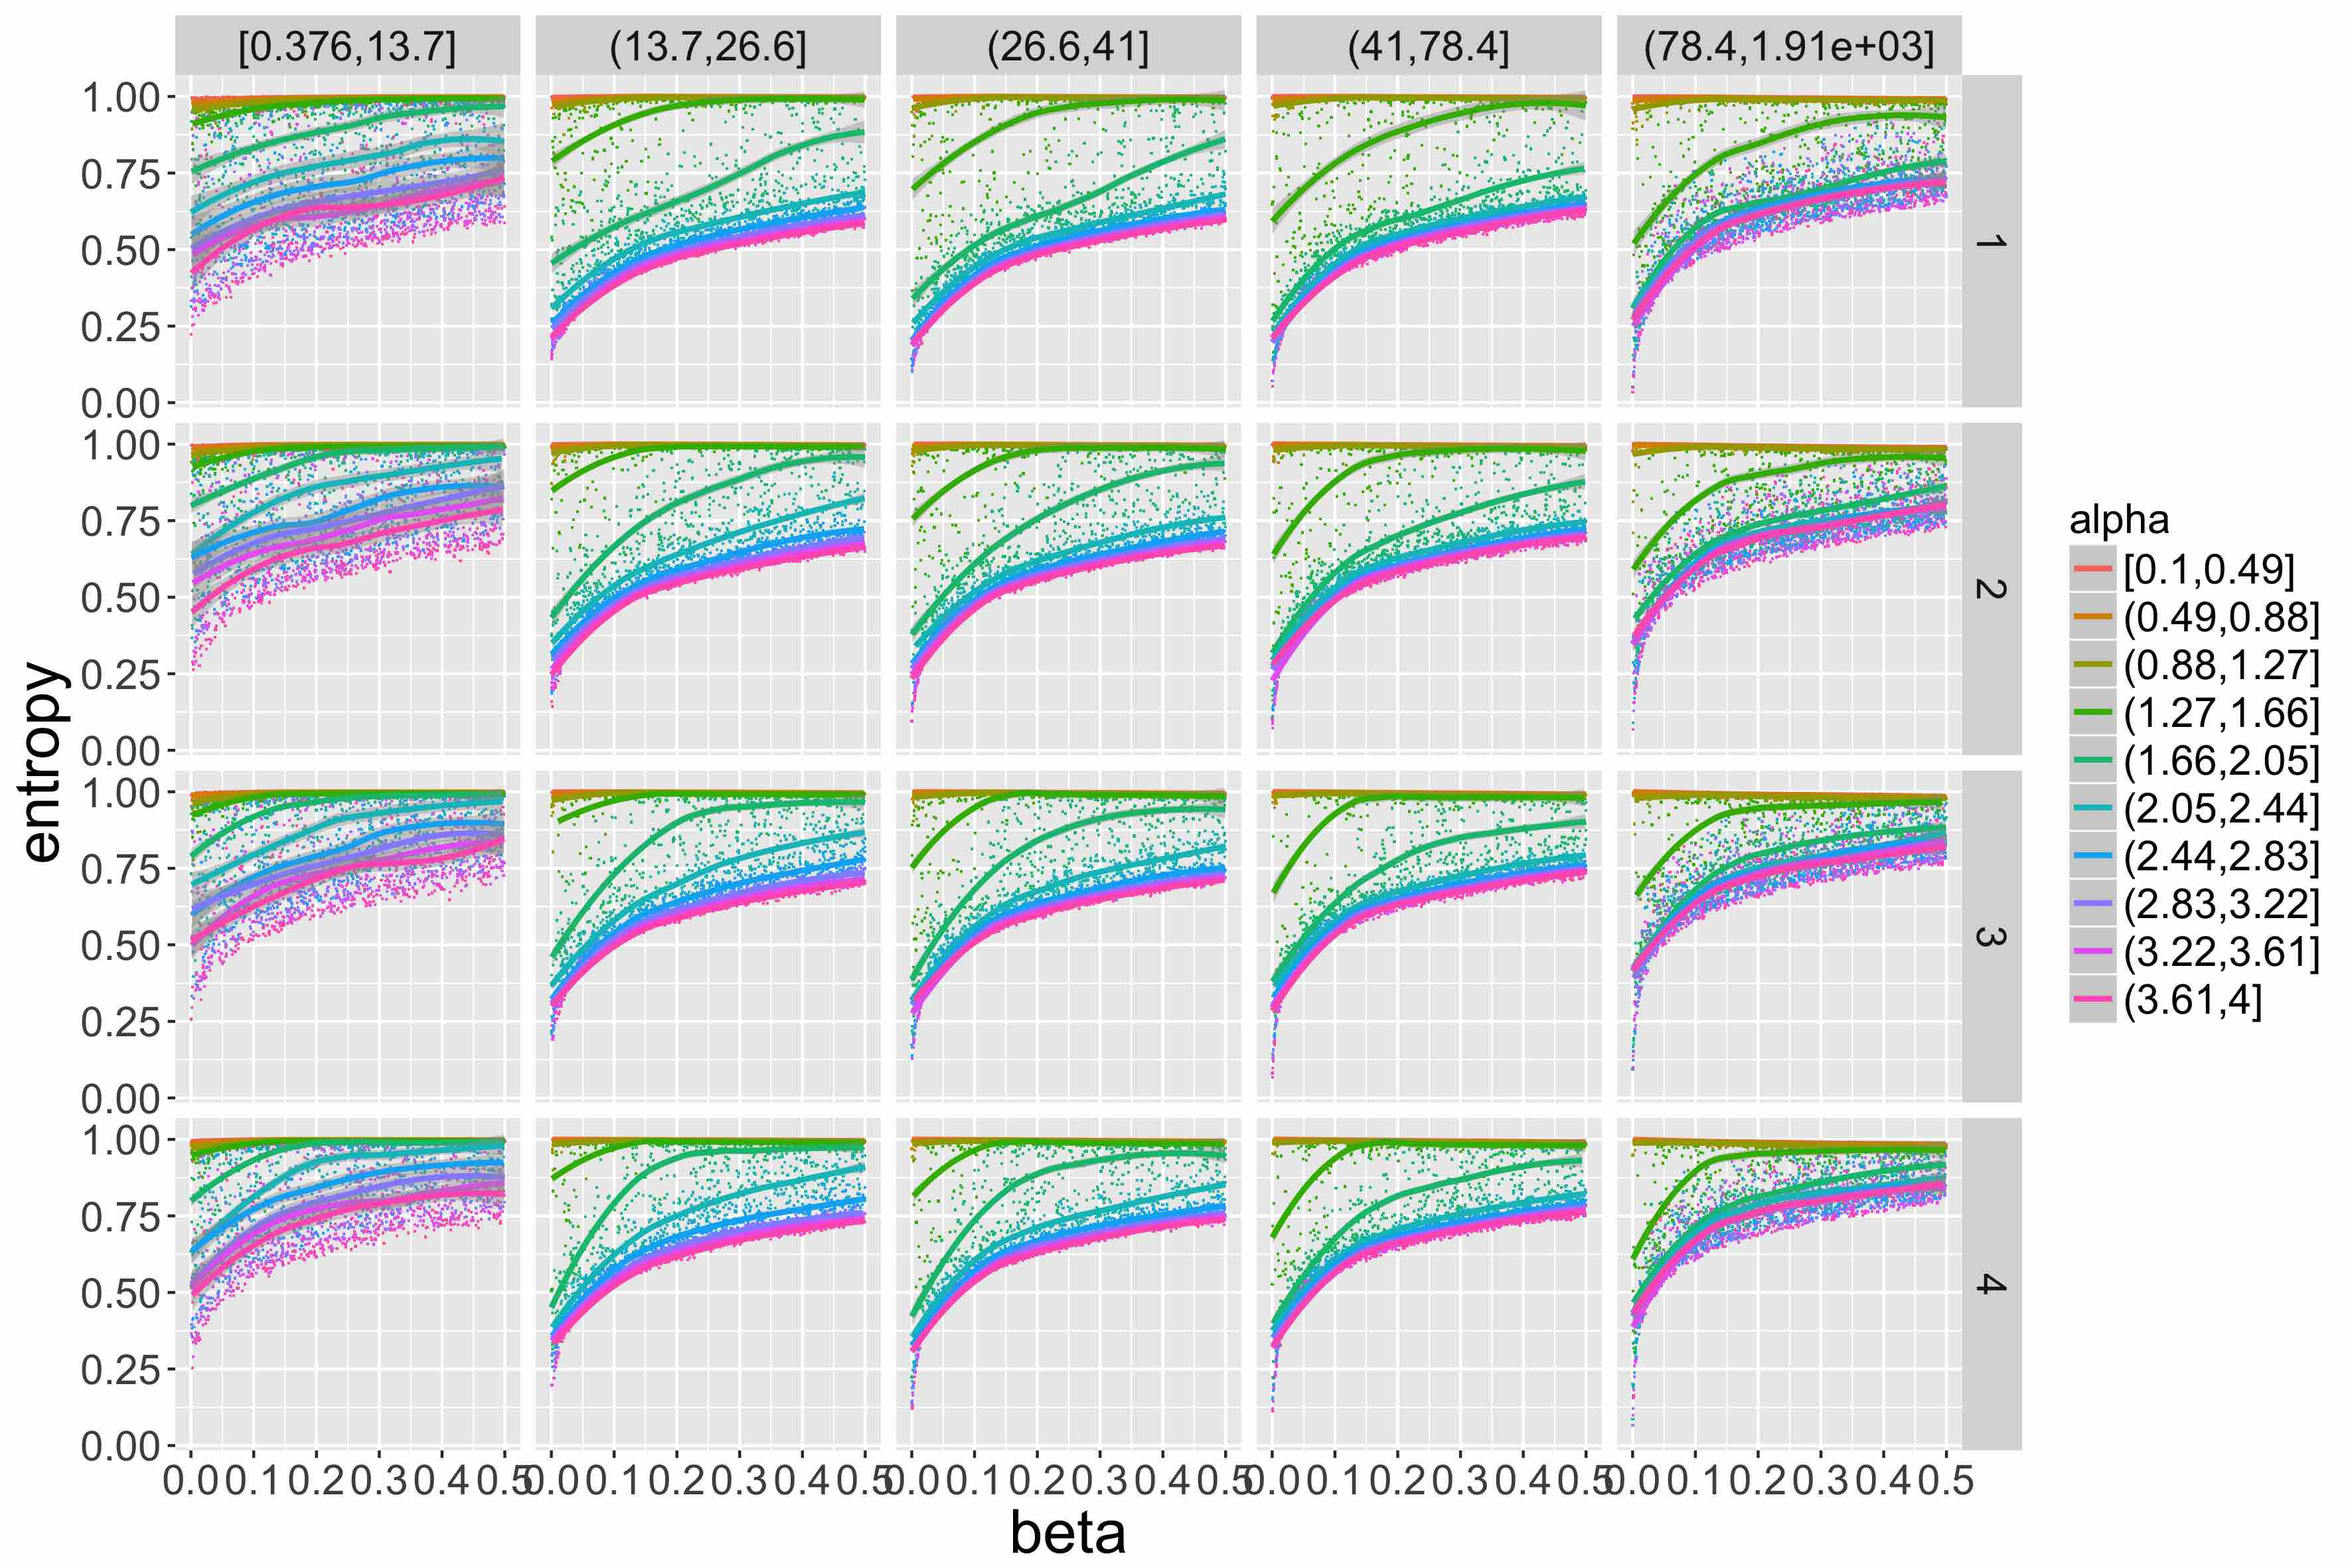
\includegraphics[width=0.8\textwidth]{Figures/Density/entropy_beta}
\caption[][]{Entropy as a function of $\alpha$ (Top) and $\beta$ (Bottom) for varying $\beta$ (resp. $\alpha$) given by color, and varying $n_d$ (rows) and $N_G$ (columns).}{}
\label{}
\end{figure}
%%%%%%%%%%%%%%%%%%%%






\subsubsection{Indicators Scatterplots}{Scatterplot des indicateurs}

% scatterplots - with real points

We show finally the full scatterplots of indicators, with real data points, in Fig.~\ref{fig:densityscatter}. These are preliminary step of the calibration on principal components, and we can see on these on which dimensions the model fails relatively to fit real data (in particular average distance).


%%%%%%%%%%%%%
\begin{figure}
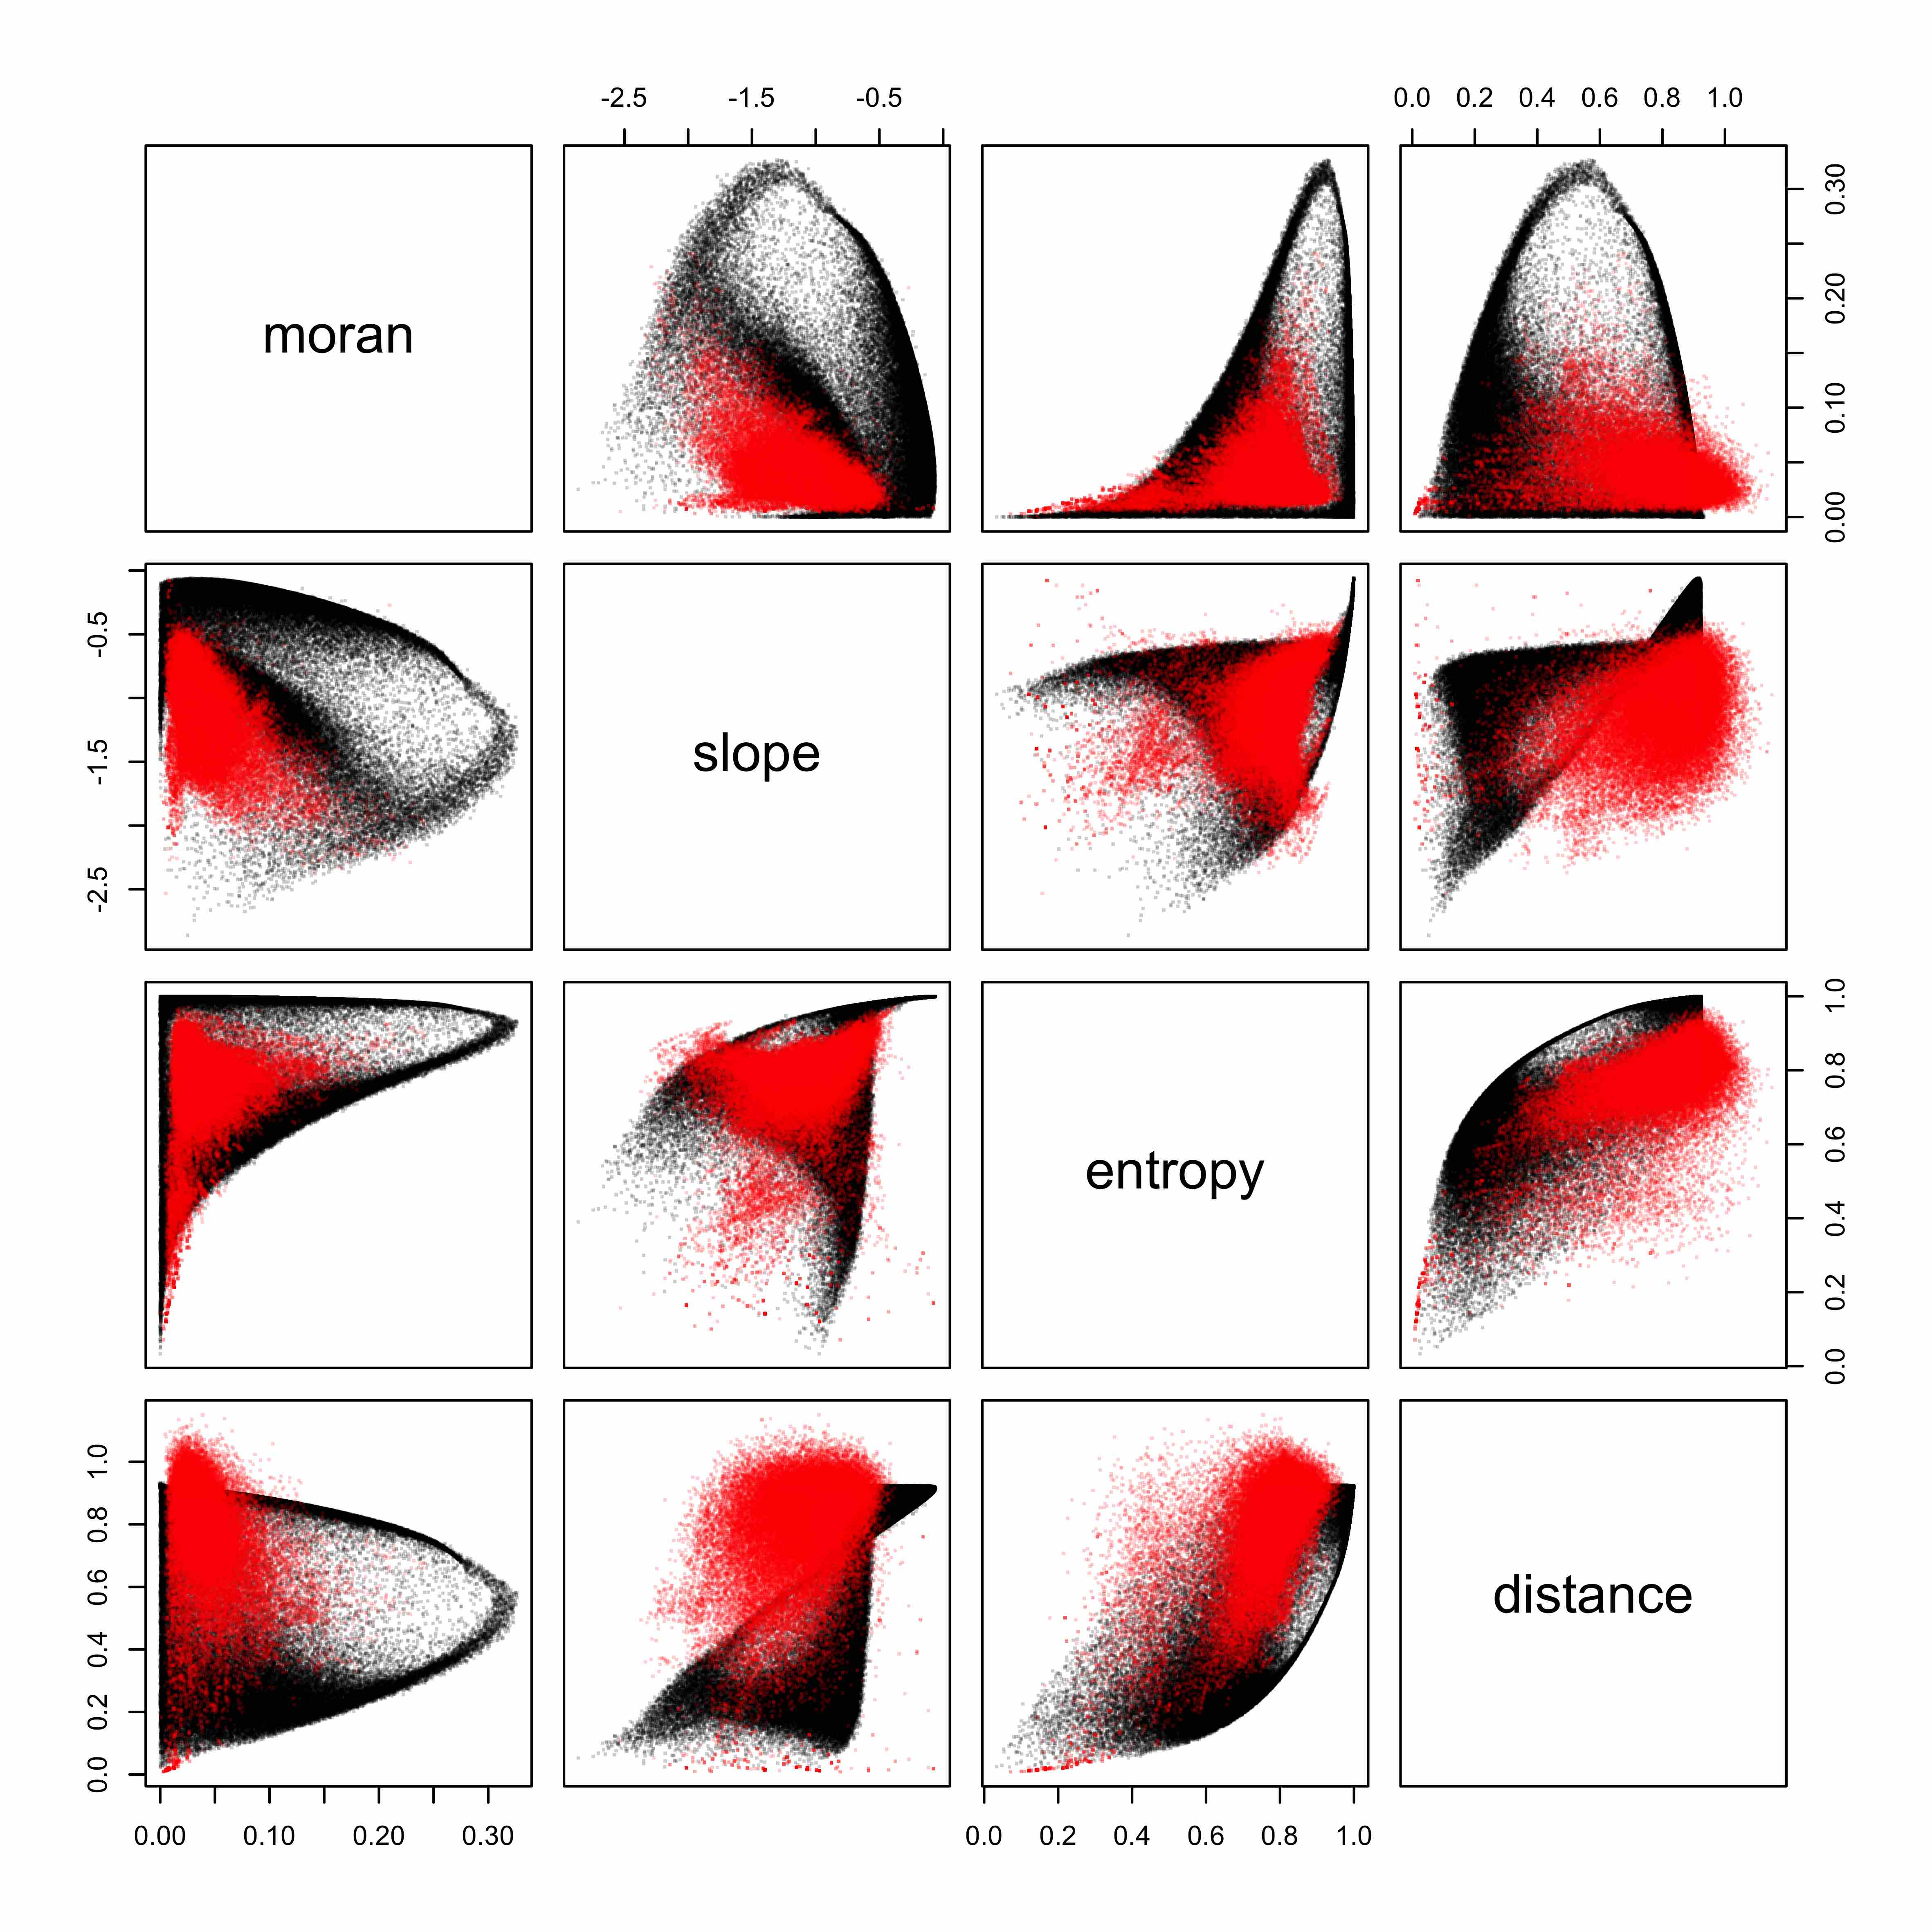
\includegraphics[width=\textwidth]{Figures/Density/scatter}
\caption[Scatter][Scatter]{Scatterplots of indicators distribution in the sampled hypercube of the parameter space. Red points correspond to real data.}{}
\label{fig:densityscatter}
\end{figure}
%%%%%%%%%%%%%





\subsection{Semi-analytical analysis of the simplified model}{Analyse semi-analytique du modèle simplifié}


\subsubsection{Partial Differential Equation}{Equation aux dérivées partielles}

We propose to derive the PDE in a simplified setting. To recall the configuration given in main text, the system has one dimension, such that $x\in \mathbb{R}$ with $1/\delta x$ cells of size $\delta x$, and we use the expected values of cell population $p(x,t) = \Eb{P(x,t)}$. We furthermore take $n_d=1$. Larger values would imply derivatives at an order higher than 2 but the following results on the existence of a stationary solution should still hold. 

Denoting $\tilde{p}(x,t)$ the intermediate populations obtained after the aggregation stage, we have

\[
\tilde{p}(x,t) = p(x,t) + N_g\cdot \frac{p(x,t)^{\alpha}}{\sum_x p(x,t)^{\alpha}}
\]

since all populations units are added independently. If $\delta x \ll 1$ then $\sum_x p^{\alpha} \simeq \int_x p(x,t)^{\alpha}dx$ and we write this quantity $P_{\alpha}(t)$. We furthermore write $p=p(x,t)$ and $\tilde{p} = \tilde{p}(x,t)$ in the following for readability.

The diffusion step is then deterministic, and for any cell not on the border ($0<x<1$), if $\delta t$ is the interval between two time steps, we have

\[
\begin{split}
p(x,t+\delta t) & = (1 - \beta) \cdot \tilde{p} + \frac{\beta}{2} \left[\tilde{p}(x-\delta x,t) + \tilde{p}(x+\delta x,t)\right]\\
& = \tilde{p} + \frac{\beta}{2} \left[\left(\tilde{p}(x+\delta x,t) - \tilde{p}\right) - \left(\tilde{p} - \tilde{p}(x-\delta x,t)\right)\right]
\end{split}
\]

Assuming the partial derivatives exist, and as $\delta x \ll 1$, we make the approximation $\tilde{p}(x+\delta x,t) - \tilde{p} \simeq \delta x\cdot \frac{\partial \tilde{p}}{\partial{x}}(x,t)$, what gives 

\[
\left(\tilde{p}(x+\delta x,t) - \tilde{p}\right) - \left(\tilde{p} - \tilde{p}(x-\delta x,t)\right) = \delta x \cdot \left(\frac{\partial \tilde{p}}{\partial{x}}(x,t) - \frac{\partial \tilde{p}}{\partial{x}}(x - \delta x,t)\right)
\]

and therefore at the second order

\[
p(x,t+\delta t) = \tilde{p} + \frac{\beta \delta x^2}{2} \cdot \frac{\partial^2 \tilde{p}}{\partial x^2}
\]

Substituting $\tilde{p}$ gives

\[
\begin{split}
\frac{\partial^2 \tilde{p}}{\partial x^2} & = \frac{\partial^2 p}{\partial x^2} + \frac{N_G}{P_\alpha}\cdot \frac{\partial}{\partial x}\left[\alpha \frac{\partial p}{\partial x} p^{\alpha - 1}\right]\\
& = \frac{\partial^2 p}{\partial x^2} + \alpha \frac{N_G}{P_\alpha} \left[\frac{\partial^2 p}{\partial x^2} p^{\alpha - 1} + (\alpha - 1) \left( \frac{\partial p}{\partial x}\right)^2 p^{\alpha - 2}\right]
\end{split}
\]

By supposing that $\frac{\partial p}{\partial t}$ exists and that $\delta t$ is small, we have $p(x,t+\delta t) - p(x,t) \simeq \delta t\frac{\partial p}{\partial t}$, what finally yields , by combining the results above, the partial differential equation


\begin{equation}\label{eq:pde}
\delta t \cdot \frac{\partial p}{\partial t} = \frac{N_G \cdot p^{\alpha}}{P_{\alpha}(t)} + \frac{\alpha \beta (\alpha - 1) \delta x^2}{2}\cdot \frac{N_G \cdot p^{\alpha-2}}{P_{\alpha}(t)} \cdot \left(\frac{\partial p}{\partial x}\right)^2 + \frac{\beta \delta x^2}{2} \cdot \frac{\partial^2 p}{\partial x^2} \cdot\left[ 1 + \alpha \frac{N_G p^{\alpha - 1}}{P_{\alpha(t)}} \right]
\end{equation}



Initial conditions should be specified as $p_0(x) = p(x,t_0)$. To have a well-posed problem similar to more classical PDE problems, we need to assume a domain and boundary conditions. A finite support is expressed by $p(x,t)=0$ for all $t$ and $x$ such that $\left|x\right|>x_m$.

%An infinite domain implies that density, in the sense of population proportion $d(x,t) = \frac{p(x,t)}{P_1(t)}$, goes to zero anywhere when time goes to infinity. Indeed, $P_1(t)=N_G\cdot t$. If $d(x,t)$ does not vanish, there exist $t_1$ such that  -> not that simple indeed


\subsubsection{Stationary solution for density}{Solution stationnaire pour la densité}

The non-linearity and the integral terms making the equation above out of the scope for analytical resolution, we study its behavior numerically in some cases. Taking a simple initial condition $p_0(0)=1$ and $p_0(x)=0$ for $x\neq 0$, we show that on a finite domain, density $d(x,t)$ always converge to a stationary solution for large $t$, for a large set of values of $(\alpha,\beta)$ with fixed $N_G=10$ ($\alpha\in \left[0.4,1.5\right]$ varying with step $0.025$ and $\log\beta \in \left[-1,-0.5\right]$ with step $0.1$). We show in Fig.~\ref{fig:stationary} the corresponding trajectories on a typical subset. The variation of the asymptotic distribution as a function of $\alpha$ and $\beta$ are not directly visible, as they depend on very low values of the outward flows at boundaries. We give in Fig.~\ref{fig:pmax} their behavior, by showing the value of the maximum of the distribution. Low values of $\beta$ give an inversion in the effect of $\alpha$, whereas high values of $\beta$ give comparable values for all $\alpha$.




%%%%%%%%%%%%%%%%%%%%
\begin{figure}[!h]
\centering
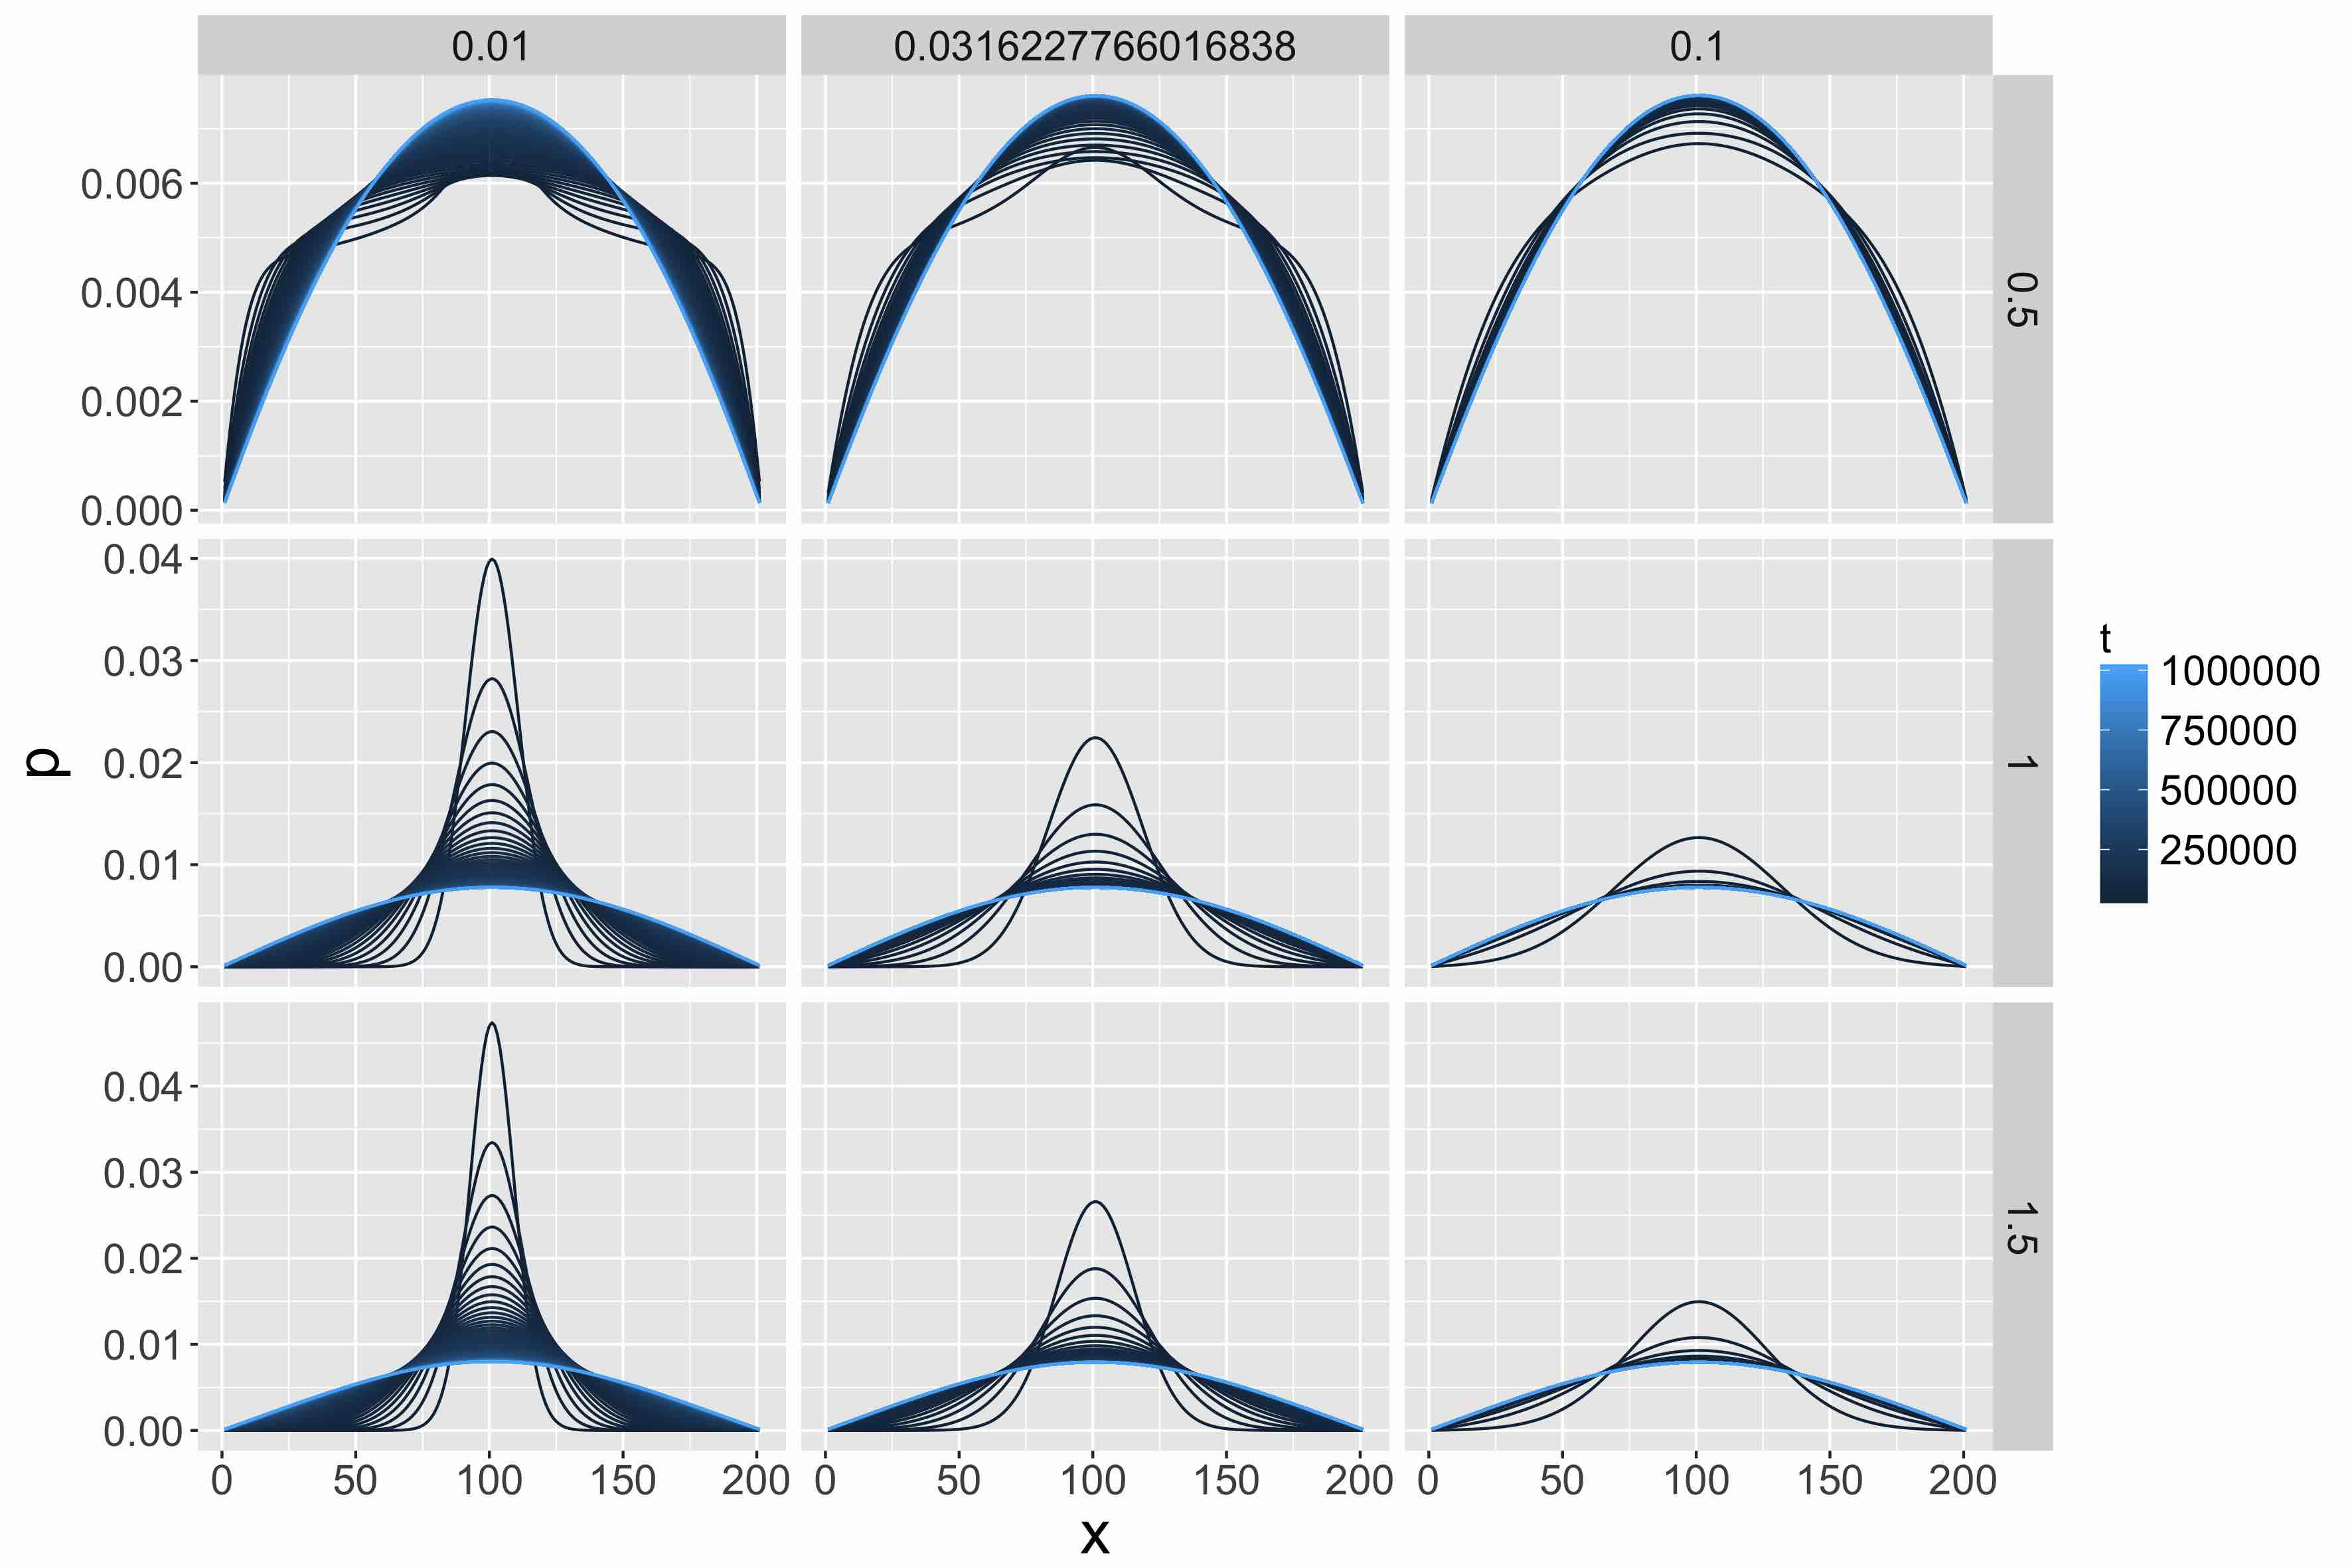
\includegraphics[width=\textwidth]{Figures/Density/stationary}
\caption[][]{Trajectories of densities as a function of the spatial dimension, for varying $\beta$ (columns) and $\alpha$ (rows). Color gives time.}{}
\label{fig:stationary}
\end{figure}
%%%%%%%%%%%%%%%%%%%%



%%%%%%%%%%%%%%%%%%%%
\begin{figure}[!h]
\centering
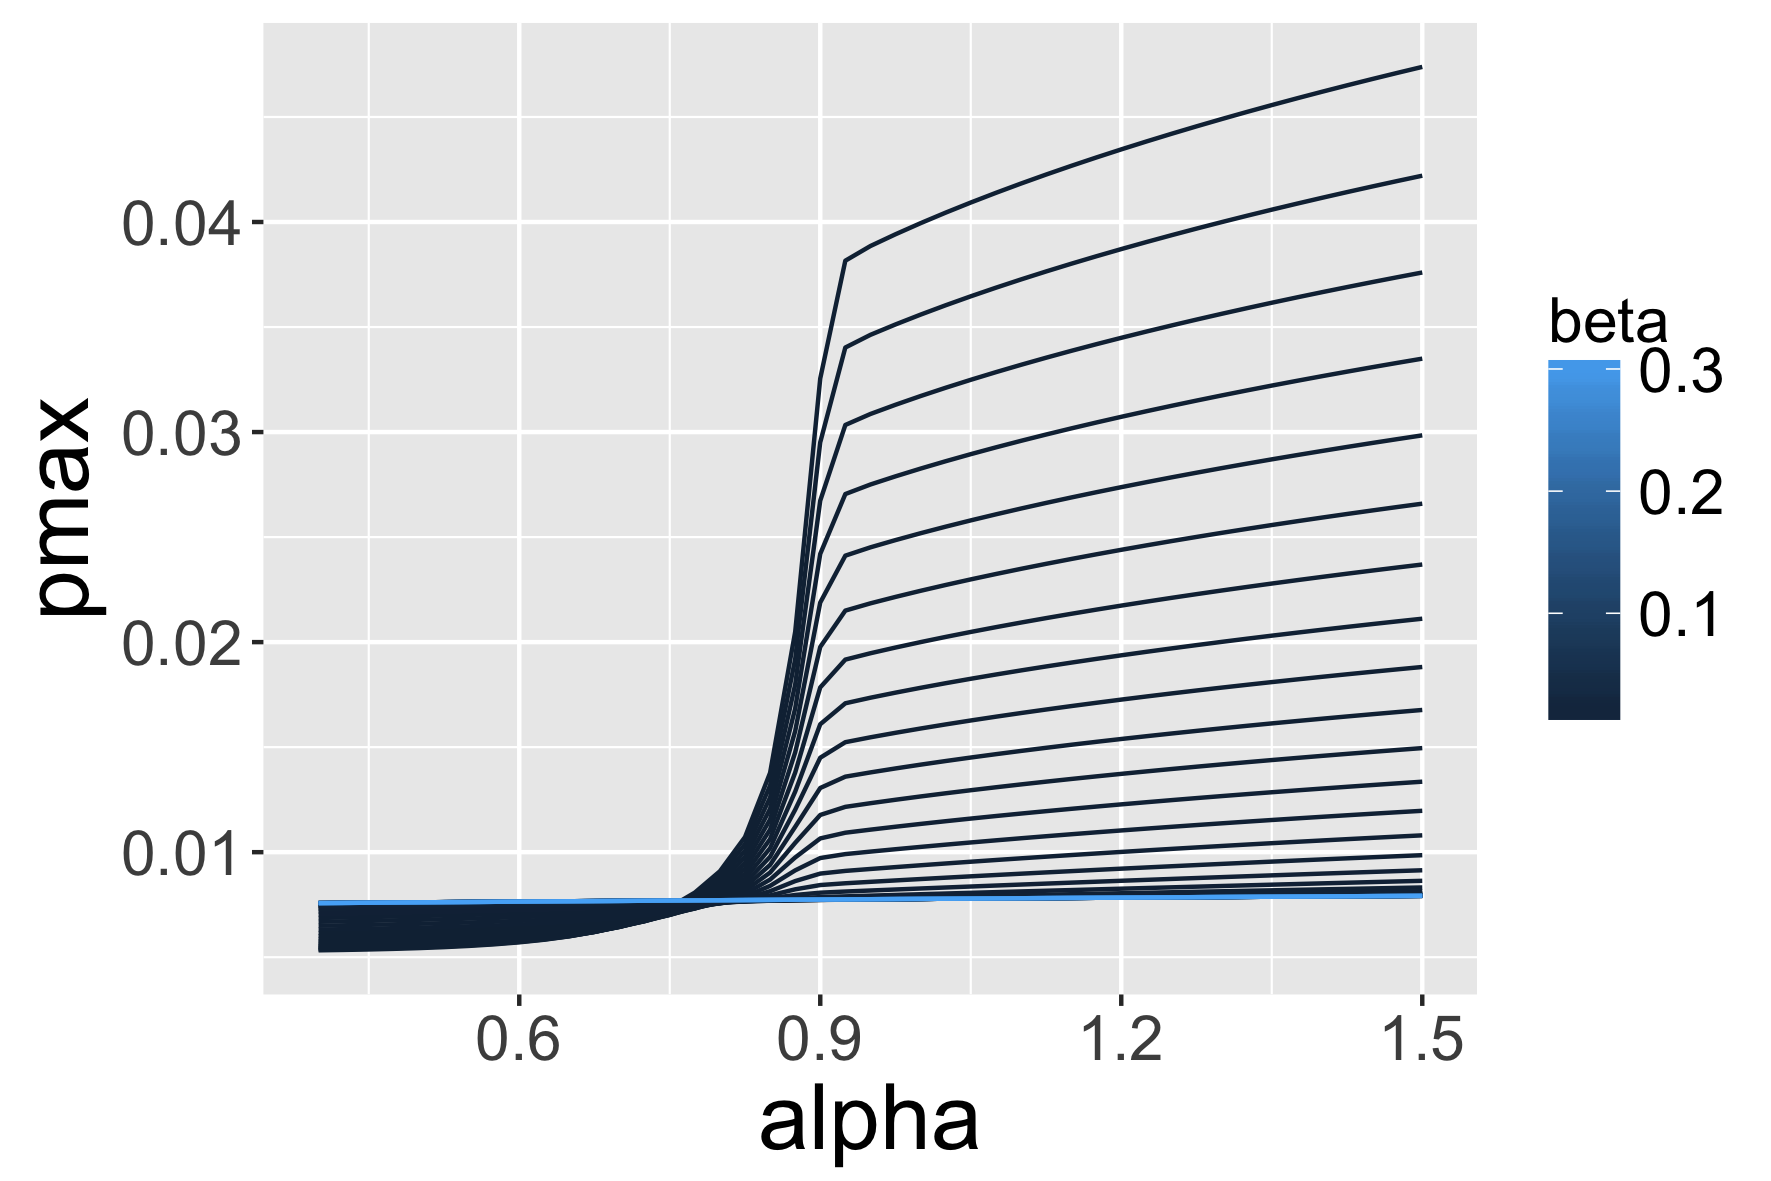
\includegraphics[width=0.49\textwidth]{Figures/Density/pmax_alpha}
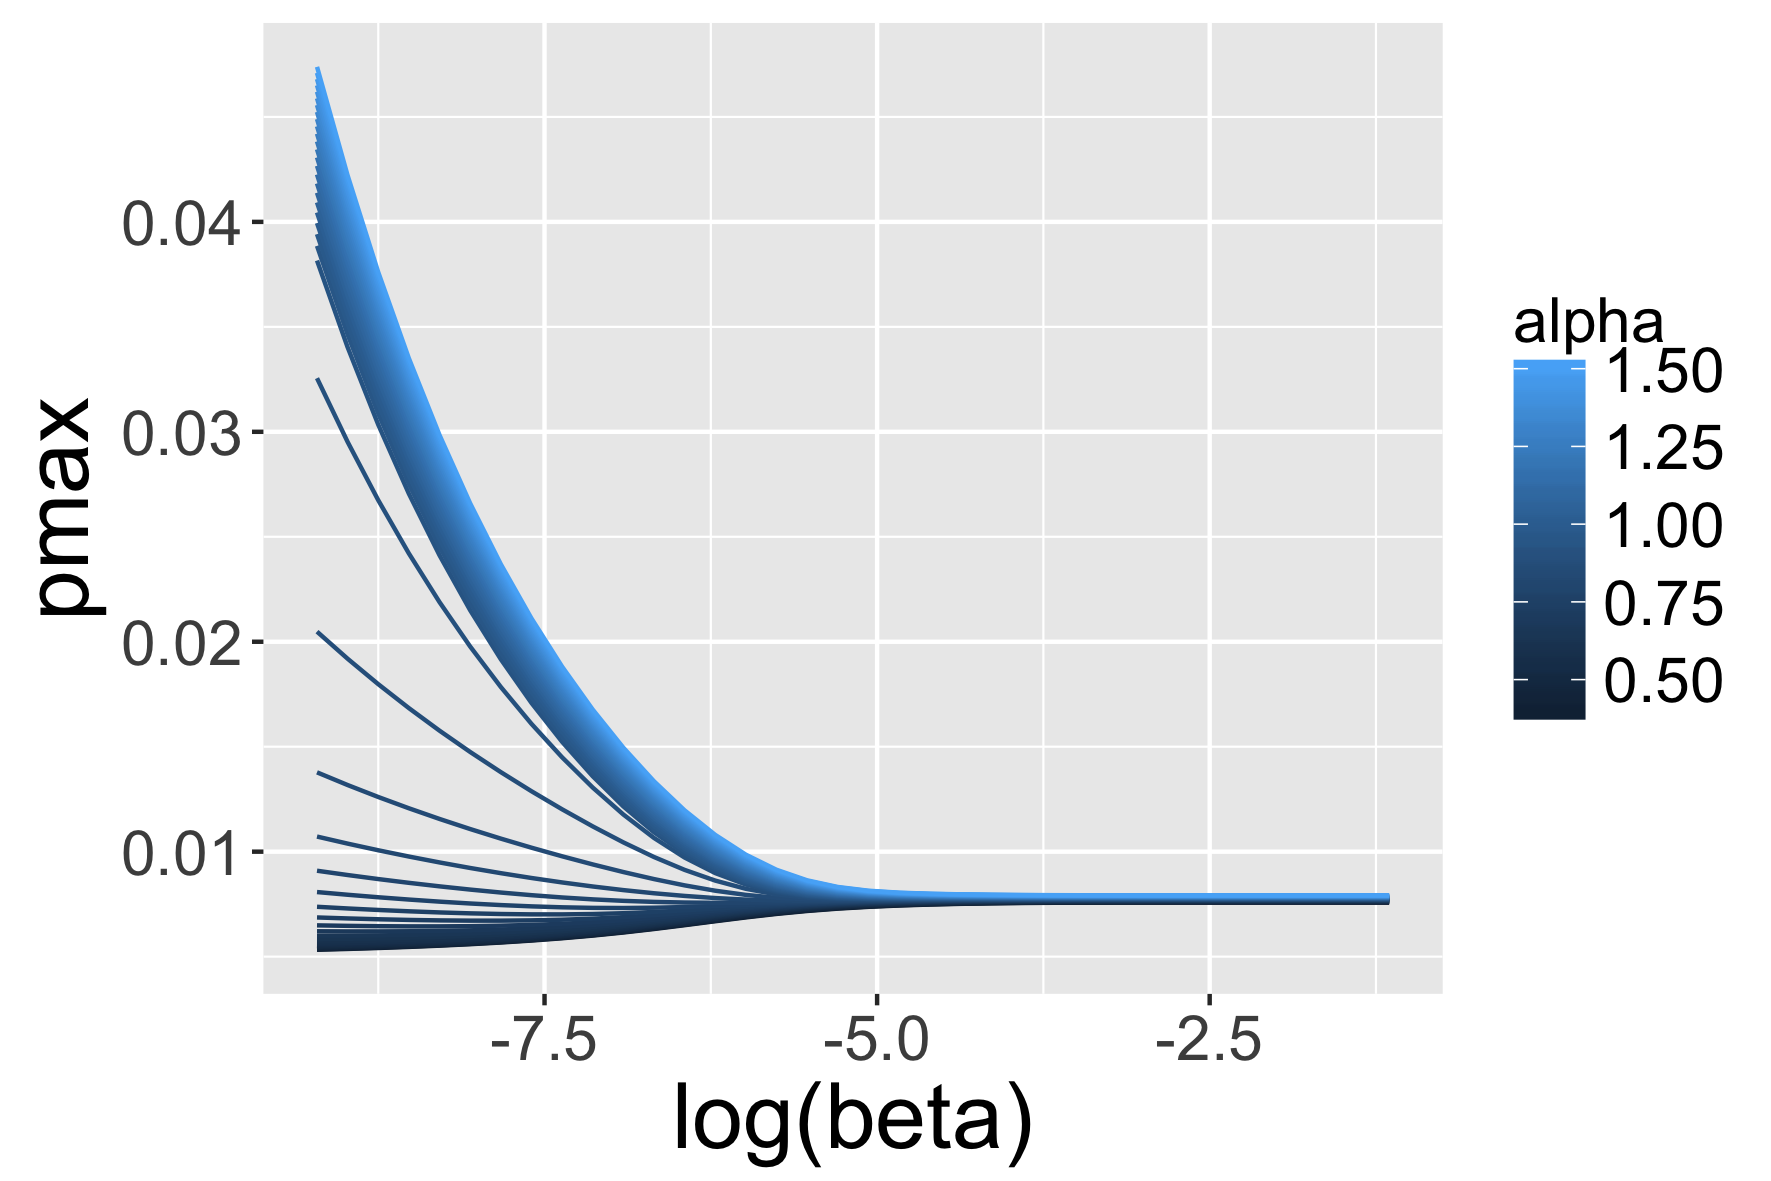
\includegraphics[width=0.49\textwidth]{Figures/Density/pmax_logbeta}
\caption[][]{Dependency of $\max d(t\rightarrow \infty )$ to $\alpha$ and $\beta$.}{}
\label{fig:pmax}
\end{figure}
%%%%%%%%%%%%%%%%%%%%







%----------------------------------------------------------------------------------------

\newpage

%%%%%%%%%%%%%%%%%%%%%%%
\section{Correlated Synthetic data}{Données Synthétiques Corrélées}

\label{app:sec:correlatedsyntheticdata}

% inclure tableaux regressions











%----------------------------------------------------------------------------------------

% -- from old empirical intro --




%One does not simply \emph{try} to model something. On that point personal experience confirms indeed that point, as I remember as an early Master student giving in to the call of incautious agent-based modeling, \comment{(Florent) pas forcément approprié dans une thèse}
% naively thinking that integrated models of any aspect of an urban system could be constructed, producing numerous NetLogo code lines to build a gaz factory with unfounded internal processes, an extremely poor external validation and no internal validation. This was a try and therefore a step towards the dark side of models bricolage. The construction of a computational model of simulation is a rigorous exercise that one can not improvise, as much as statistical modeling. Recent progresses in the field~\cite{banos2013pour} help to that purpose, and modular model construction and validation is one tool useful to avoid becoming lost in shady places.

%We propose in this chapter simple modeling experiments, conceived to be preliminaries for more elaborated tests of our theory. We begin with a simple diffusion-aggregation model of urban growth as a relatively small scale. Beginning with simple assumptions does not mean a non-rigorous exploration of the model, that is therefore explored and calibrated on real data. The fact that we reproduce existing urban forms \comment{(Florent) oui mais ce n'est pas du tout un problème pour ta thèse. Ta thèse porte sur FU $\leftrightarrow$ Réseaux ; le fait qu'on puisse faire des modèles forme urbaine purs (avec mécanismes abstraits) et idem pour les réseaux d'ailleurs ne change rien à l'affaire. tout tes modèles ne doivent pas viser à reproduire FU \& réseau mais à reproduire FU $\leftrightarrow$ Réseaux}
% without the use of networks suggest either the total absence of network influence at this scale, or its very strong influence yielding apparent random effects that disappear in average calibration. We propose then to simply couple this model with a network generation heuristic in order to study feasible correlations between morphology and network. The absence of coupled calibration \comment{(Florent) pourquoi ? remarque tu dis le contraire là ?}
%  avoids to draw empirical conclusion but the method is satisfying in itself as it permits the generation of synthetic territorial configurations where correlation structure is controlled. We finally describe a project of benchmark of diverse heuristic models for network generation.





